%Input preamble
%Style
\documentclass[12pt]{article}
\usepackage[top=1in, bottom=1in, left=1in, right=1in]{geometry}
\parindent 22pt
\usepackage{fancyhdr}

%Packages
\usepackage{adjustbox}
\usepackage{amsmath}
\usepackage{amsfonts}
\usepackage{amssymb}
\usepackage{bm}
\usepackage[table]{xcolor}
\usepackage{tabu}
\usepackage{color,soul}
\usepackage{makecell}
\usepackage{longtable}
\usepackage{multirow}
\usepackage[normalem]{ulem}
\usepackage{etoolbox}
\usepackage{graphicx}
\usepackage{tabularx}
\usepackage{ragged2e}
\usepackage{booktabs}
\usepackage{caption}
\usepackage{fixltx2e}
\usepackage[para, flushleft]{threeparttablex}
\usepackage[capposition=top,objectset=centering]{floatrow}
\usepackage{subcaption}
\usepackage{pdfpages}
\usepackage{pdflscape}
\usepackage{natbib}
\usepackage{bibunits}
\definecolor{maroon}{HTML}{990012}
\usepackage[colorlinks=true,linkcolor=maroon,citecolor=maroon,urlcolor=maroon,anchorcolor=maroon]{hyperref}
\usepackage{marvosym}
\usepackage{makeidx}
\usepackage{tikz}
\usetikzlibrary{shapes}
\usepackage{setspace}
\usepackage{enumerate}
\usepackage{rotating}
\usepackage{tocloft}
\usepackage{epstopdf}
\usepackage[titletoc]{appendix}
\usepackage{framed}
\usepackage{comment}
\usepackage{xr}
\usepackage{titlesec}
\usepackage{footnote}
\usepackage{longtable}
\newlength{\tablewidth}
\setlength{\tablewidth}{9.3in}
\setcounter{secnumdepth}{4}

\titleformat{\paragraph}
{\normalfont\normalsize\bfseries}{\theparagraph}{1em}{}
\titlespacing*{\paragraph}
{0pt}{3.25ex plus 1ex minus .2ex}{1.5ex plus .2ex}
\makeatletter
\pretocmd\start@align
{%
  \let\everycr\CT@everycr
  \CT@start
}{}{}
\apptocmd{\endalign}{\CT@end}{}{}
\makeatother
%Watermark
\usepackage[printwatermark]{xwatermark}
\usepackage{lipsum}
\definecolor{lightgray}{RGB}{220,220,220}
%\newwatermark[allpages,color=lightgray,angle=45,scale=3,xpos=0,ypos=0]{Preliminary Draft}

%Further subsection level
\usepackage{titlesec}
\setcounter{secnumdepth}{4}
\titleformat{\paragraph}
{\normalfont\normalsize\bfseries}{\theparagraph}{1em}{}
\titlespacing*{\paragraph}
{0pt}{3.25ex plus 1ex minus .2ex}{1.5ex plus .2ex}

\setcounter{secnumdepth}{5}
\titleformat{\subparagraph}
{\normalfont\normalsize\bfseries}{\thesubparagraph}{1em}{}
\titlespacing*{\subparagraph}
{0pt}{3.25ex plus 1ex minus .2ex}{1.5ex plus .2ex}

%Functions
\DeclareMathOperator{\cov}{Cov}
\DeclareMathOperator{\corr}{Corr}
\DeclareMathOperator{\var}{Var}
\DeclareMathOperator{\plim}{plim}
\DeclareMathOperator*{\argmin}{arg\,min}
\DeclareMathOperator*{\argmax}{arg\,max}

%Math Environments
\newtheorem{theorem}{Theorem}
\newtheorem{claim}{Claim}
\newtheorem{condition}{Condition}
\renewcommand\thecondition{C--\arabic{condition}}
\newtheorem{algorithm}{Algorithm}
\newtheorem{assumption}{Assumption}
\renewcommand\theassumption{A--\arabic{assumption}}
\newtheorem{remark}{Remark}
\renewcommand\theremark{R--\arabic{remark}}
\newtheorem{definition}[theorem]{Definition}
\newtheorem{hypothesis}[theorem]{Hypothesis}
\newtheorem{property}[theorem]{Property}
\newtheorem{example}[theorem]{Example}
\newtheorem{result}[theorem]{Result}
\newenvironment{proof}{\textbf{Proof:}}{$\bullet$}

%Commands
\newcommand\independent{\protect\mathpalette{\protect\independenT}{\perp}}
\def\independenT#1#2{\mathrel{\rlap{$#1#2$}\mkern2mu{#1#2}}}
\newcommand{\overbar}[1]{\mkern 1.5mu\overline{\mkern-1.5mu#1\mkern-1.5mu}\mkern 1.5mu}
\newcommand{\equald}{\ensuremath{\overset{d}{=}}}
\captionsetup[table]{skip=10pt}
%\makeindex

\setlength\parindent{20pt}
\setlength{\parskip}{0pt}

\newcolumntype{L}[1]{>{\raggedright\let\newline\\\arraybackslash\hspace{0pt}}m{#1}}
\newcolumntype{C}[1]{>{\centering\let\newline\\\arraybackslash\hspace{0pt}}m{#1}}
\newcolumntype{R}[1]{>{\raggedleft\let\newline\\\arraybackslash\hspace{0pt}}m{#1}}



%Logo
%\AddToShipoutPictureBG{%
%  \AtPageUpperLeft{\raisebox{-\height}{
\includegraphics[width=1.5cm]{uchicago.png}}}
%}

\newcolumntype{L}[1]{>{\raggedright\let\newline\\\arraybackslash\hspace{0pt}}m{#1}}
\newcolumntype{C}[1]{>{\centering\let\newline\\\arraybackslash\hspace{0pt}}m{#1}}
\newcolumntype{R}[1]{>{\raggedleft\let\newline\\\arraybackslash\hspace{0pt}}m{#1}}

\newcommand{\mr}{\multirow}
\newcommand{\mc}{\multicolumn}

%\newcommand{\comment}[1]{}

%Other parameters
\newcommand{\noutcomes}{95}
\newcommand{\noutcomesexpp}{357}
\newcommand{\noutcomesexpm}{343}
\newcommand{\noutcomesexpf}{355}
\newcommand{\treatsubsabc}{$75\%$}
\newcommand{\treatsubscarec}{$74\%$}
\newcommand{\treatsubscaref}{$63\%$}

%Counts
%Males
\newcommand{\positivem}{$78\%$}
\newcommand{\positivesm}{$29\%$}

%Females
\newcommand{\positivef}{$78\%$}
\newcommand{\positivesf}{$31\%$}

%Counts, control substitution
%Males
\newcommand{\positivecsnm}{$47\%$}
\newcommand{\positivescsnm}{$15\%$}

\newcommand{\positivecsam}{$79\%$}
\newcommand{\positivescsam}{$29\%$}

%Females
%% no alternative
\newcommand{\positivecsnf}{$84\%$}
\newcommand{\positivescsnf}{$55\%$}

%% alternative
\newcommand{\positivecsaf}{$79\%$}
\newcommand{\positivescsaf}{$33\%$}

%Pooled

%Effects
%Males

%Females
\newcommand{\empf}{$8$}
\newcommand{\yearsedf}{$1.7$}



%Pooled

%CBA
%IRR
%Males
\newcommand{\irrm}{$15\%$}
\newcommand{\irrsem}{$5\%$}

%Females
\newcommand{\irrf}{$9\%$}
\newcommand{\irrsef}{$7\%$}

%Pooled
\newcommand{\irrp}{$13\%$}
\newcommand{\irrsep}{$5\%$}

%BC
%Males
\newcommand{\bcm}{$11.24$}
\newcommand{\bcsem}{$4.60$}

%Females
\newcommand{\bcf}{$2.35$}
\newcommand{\bcsef}{$1.09$}

%Pooled
\newcommand{\bcp}{$5.63$}
\newcommand{\bcsep}{$2.15$}

%NPV streams
%Pooled
\newcommand{\parincomenpvp}{$\$119,346$}

\newcommand*\leftright[2]{%
  \leavevmode
  \rlap{#1}%
  \hspace{0.5\linewidth}%
  #2}

\newcommand{\orth}{\ensuremath{\perp\!\!\!\perp}}%
\newcommand{\indep}{\orth}%
\newcommand{\notorth}{\ensuremath{\perp\!\!\!\!\!\!\diagup\!\!\!\!\!\!\perp}}%
\newcommand{\notindep}{\notorth}

\externaldocument{abc_comprehensivecba_appendix}
\pagenumbering{roman}

\begin{document}

\begin{titlepage}

\title{\Large \textbf{The Life-cycle Benefits of an Influential Early Childhood Program}\thanks{This research was supported in part by the American Bar Foundation; the Pritzker Children's Initiative, the Buffett Early Childhood Fund, National Institutes of Health grants NICHD R37HD065072, NICHD R01HD54702, NIA R24AG048081, P30AG024968, an anonymous funder, Successful Pathways from School to Work, an initiative of the University of Chicago's Committee on Education funded by the Hymen Milgrom Supporting Organization, and the Human Capital and Economic Opportunity Global Working Group, an initiative of the Center for the Economics of Human Development, affiliated with the Becker Friedman Institute for Research in Economics, and funded by the Institute for New Economic Thinking. The views expressed in this paper are solely those of the authors and do not necessarily represent those of the funders or the official views of the National Institutes of Health. Collaboration with Yu Kyung Koh, Sylvi Kuperman, Stefano Mosso, Rodrigo Pinto, Joshua Shea, Jake Torcasso, and Anna Ziff on related work has strengthened the analysis in this paper. Collaboration with Bryan Tysinger on adapting the Future America Model is gratefully acknowledged. For helpful comments, we thank St\'{e}phane Bonhomme, Fl\'{a}vio Cunha, Steven Durlauf, Sidhart Moktan, Azeem Shaikh, Matthew Tauzer, and Ed Vytlacil. For information on the implementation of the Carolina Abecedarian Project and the Carolina Approach to Responsive Education and assistance in data acquisition, we thank Peg Burchinal, Carrie Bynum, Frances Campbell, and Elizabeth Gunn. For information on childcare in North Carolina, we thank Richard Clifford and Sue Russell. The Web Appendix for this paper can be found at \url{http://cehd.uchicago.edu/ABC_CARE}.}}

\author{
Jorge Luis Garc\'{i}a\\
The University of Chicago \and
James J. Heckman \\
American Bar Foundation \\
The University of Chicago \and
Andr\'{e}s Hojman \\
The University of Chicago \\ \and
Duncan Ermini Leaf \\
University of Southern California \and
Mar\'{i}a Jos\'{e} Prados \\
University of Southern California}
\date{First Draft: January 5, 2016\\ This Draft: \today}

\maketitle

\end{titlepage}

\newgeometry{top=.8in, bottom=.8in, left=.8in, right=.8in}
\singlespacing

\begin{abstract}
This paper estimates the diverse array of life-cycle benefits of an influential early childhood program targeted to disadvantaged children and their families. The program is a prototype for numerous interventions currently in place around the world. It is evaluated by random assignment and follows participants through their mid-30s. It has substantial beneficial long-term effects on (a) health and the quality of life, (b) the labor incomes of participants, (c) crime, (d) education, and (e) the labor incomes of the mothers of the participants through subsidizing their childcare. There are benefits across the life cycle for both genders, but substantially greater monetized benefits for boys. The overall rate of return and benefit/cost ratio are economically and statistically significant: 13\% per annum and 5.6 respectively. These estimates account for the welfare costs of taxation to finance the program and survive a variety of sensitivity analyses.
\end{abstract}

\noindent \textbf{Keywords}: Childcare, crime, early childhood education, gender differences in responses to programs, health, long-term predictions, quality of life, randomized trials \\
\noindent \textbf{JEL codes}: J13, I28, C93


\tableofcontents
%\listoffigures
%\listoftables
\restoregeometry

\clearpage
\doublespacing

\setcounter{page}{0}
\pagenumbering{arabic}

\section{Introduction}

This paper documents the diverse array of life-cycle benefits of an influential early childhood program targeted to disadvantaged children. The program has substantial impacts on the lives of participants. Monetizing benefits and costs across multiple domains, we estimate a rate of return of 13\% per annum and a benefit/cost ratio of 5.6. There are substantial differences in monetized benefits across genders, favoring boys.

Our analysis contributes to a growing literature on the benefits of early programs for disadvantaged children.\footnote{See, e.g., \cite{Currie_2011_AER} and \cite{Elango_Hojman_etal_2016_Early-Edu}.} Long-term evidence on their effectiveness is surprisingly limited.\footnote{The major source of evidence is from the Perry Preschool Program (see \citealp{Schweinhart_Montie_ea_2005_BOOKlifetime} and \citealp{Heckman_Moon_etal_2010_RateofReturn,Heckman_Moon_etal_2010_QE}), the Carolina Abecedarian Project (ABC) and the Carolina Approach to Responsive Education (CARE) (\citealp{Ramey_Campbell_etal_2000_ADS,Ramey-etal_2012-ABC}), and the Infant Health and Development Program (IHDP) (\citealp{Gross_Spiker_etal_1997_BOOKHelpinglowbirth,Duncan_Sojourner_2013_JHR}). IHDP was inspired by ABC/CARE \citep[][]{Gross_Spiker_etal_1997_BOOKHelpinglowbirth}.} For want of long-term followup data, many studies of early childhood programs report outcomes at early ages. Moreover, they use only limited sets of outcomes like IQ or scores on school readiness measures.\footnote{See, e.g., \cite{Kline_Walters_2016_QJE} and \cite{Weiland_2013_CD_Impacts-of-Pre-K}.} Yet it is the long-term costs and benefits across multiple domains of life that are relevant for policy analysis.

We analyze a large array of long-term benefits through the mid-30s from two virtually identical early childhood programs with randomized designs conducted in North Carolina. The programs are the Carolina Abecedarian Project (ABC) and the Carolina Approach to Responsive Education (CARE), henceforth ABC/CARE. They were launched in the early 1970s and have long-term follow-ups through age 34. The programs started early (at 8 weeks of life) and engaged participants to age 5. We analyze their impacts on a variety of life-relevant outcomes such as health, the quality of life, participation in crime, labor income, IQ, schooling, and increases in mothers' labor income arising from program subsidies to childcare.

Evidence from these programs is relevant for contemporary policy discussions because their main components are present in a variety of programs currently in place around the world.\footnote{Programs inspired by ABC/CARE have been (and are being) launched around the world. \citet{Sparling_2010_Highlights} and \citet{Ramey_Ramey_Lanzi_2014_Interventions} list numerous programs based on ABC/CARE. The names of the programs with years launched and locations in parentheses are: IHDP---eight different cities around the U.S. \citep{Spiker-etal_1997_Helping}; Early Head Start and Head Start in the U.S. \citep{Schneider_McDonald-eds_2007_Scale-Up_Vol-1}; John's Hopkins Cerebral Palsy Study in the U.S. \citep{Sparling_2010_Highlights}; Classroom Literacy Interventions and Outcomes (CLIO) study in the U.S. \citep{Sparling_2010_Highlights}; Massachusetts Family Child Care Study \citep{Collins_etal_2010_Massachusetts-Study}; Healthy Child Manitoba Evaluation \citep{Healthy_Child_Manitoba_2015_Starting-Early}; Abecedarian Approach within an Innovative Implementation Framework \citep{Jensen_Nielsen_2016_ABC-Programme-Pilot}; and Building a Bridge into Preschool in Remote Northern Territory Communities in Australia \citep{UMonash_Dataset_2015_URL}. Educare programs are also based on ABC/CARE \citep{Educare_2014_Research_Agenda,Yazejian_Bryant_2012_Educare}.} About 19\% of all African-American children are eligible for the program today.\footnote{43\% of African-American children were eligible in 1972 \citep{Garcia_2016_National-Implementation-ECI}.}

Summarizing the benefits of a program with a diverse array of outcomes across many domains and periods of life is both challenging and rewarding. Doing so highlights the numerous ways through which early childhood programs enhance capabilities. We use a variety of methodologies to characterize program benefits. Instead of reporting only individual treatment effects or categories of treatment effects, our benefit/cost analysis accounts for all program components, including the welfare costs of taxes to publicly finance the program.\footnote{\cite{Barnett_Masse_2002_benefitcost,Barnett_Masse_2007_EER} present a cost/benefit analysis for ABC through age 21, before many benefits are realized. They report a benefit/cost ratio of 2.5, but give no standard error or sensitivity analyses for their estimate. They do not disaggregate by gender. For want of the data collected on health at age 34, they do not account for health benefits. They use self-reported crime data (unlike the administrative crime data later collected that we analyze) and ignore the welfare costs of financing the program. We use cost data from primary sources not available to them.}

A fundamental problem facing the evaluation of any human capital program is assessing out of sample future benefits of the program. Most solutions to this problem are based on versions of a synthetic cohort approach using the adjusted outcomes of older cohorts comparable to treated individuals to proxy treatment effects.\footnote{\cite{Mincer_1974_schooling} addresses this problem using a synthetic cohort approach and provides evidence on its validity. See the discussion of the synthetic cohort approach in \cite{Heckman_Lochner_ea_2006_HEE}.} We address this problem by using a variety of sources of information up to age 34, combined with information from multiple panel data sources to predict benefits and costs over the lifetimes of participants.\footnote{\citet{Ridder_Moffitt_2007_hbk_metricsdata} provide a valuable discussion of data pooling methods. These methods are related to the older ``surrogate marker'' literature in biostatistics (see e.g., \citealp{Prentice_1989_Surrogate_SiM}).}

A sufficient condition for making unbiased out-of-sample predictions (and for being able to test this condition) is that program treatment effects arise as changes in inputs in a stable (across treatment regimes) production function. Evidence supporting this assumption is given in \citet{Heckman_Pinto_etal_2013_PerryFactor} and \cite{Attanasio-etal_2015_NBER_Estimating-Production}. We test and do not reject this assumption in this paper.\footnote{An appealing feature of our test is that it is based on larger sample. We perform it across multiple data sources. See Appendix{appendix:pred} for details.}

We account for sampling uncertainty from pooling data and conduct sensitivity analyses for outcomes for which sampling uncertainty is not readily quantified. Our approach to pooling multiple data sets and analyzing blocks of outcomes is of interest in its own right as a template for evaluating other programs with numerous long-run outcomes using intermediate outcome measures.

Another major methodological challenge we confront is control group substitution bias.\footnote{See \cite{Heckman_1992_randomization}, \cite{Heckman_Hohmann_etal_2000_QJE}, and \cite{Kline_Walters_2016_QJE}.} Roughly 75\% of the control groups in ABC/CARE take some form of alternative preschool at least some of the time. We define and estimate parameters accounting for the variety of choices available and taken by the control groups in our study.

We contribute to the literature on the effectiveness of early childhood programs by considering long-term benefits on health. We estimate the savings in life-cycle medical costs and improvements in the quality of life.\footnote{\cite{Campbell_Conti_etal_2014_EarlyChildhoodInvestments} show the substantial adult (age 34) health benefits of ABC but do not present a cost/benefit analysis of their results.} We also find substantial childcare benefits that promote work by the mothers of participants, and additional benefits for participants in terms of reduced crime, gains in life-cycle labor income, reduced special education costs, and enhanced educational attainment.

Figure~\ref{figure:npvsall} summarizes the main finding of this paper. It displays the discounted (by a 3\% discount rate) life-cycle program (net) costs and benefits (in 2014 USD) for a pooled sample of male and female participants along with the monetized benefits disaggregated by category. Costs are substantial, as has frequently been noted by critics.\footnote{See, e.g., \citet{Whitehurst_2014_Senate_Testimony} and \citet{Fox_News_2014_Head_Start_Effects}.} But so are the benefits, which far outweigh the costs. The benefits accrue accross multiple life domains.

\begin{sidewaysfigure}[!htbp]
\caption{Net Present Value of Main Components of the Cost/benefit Analysis Over the Life-cycle, ABC/CARE Males and Females}
\label{figure:npvsall}
\centering
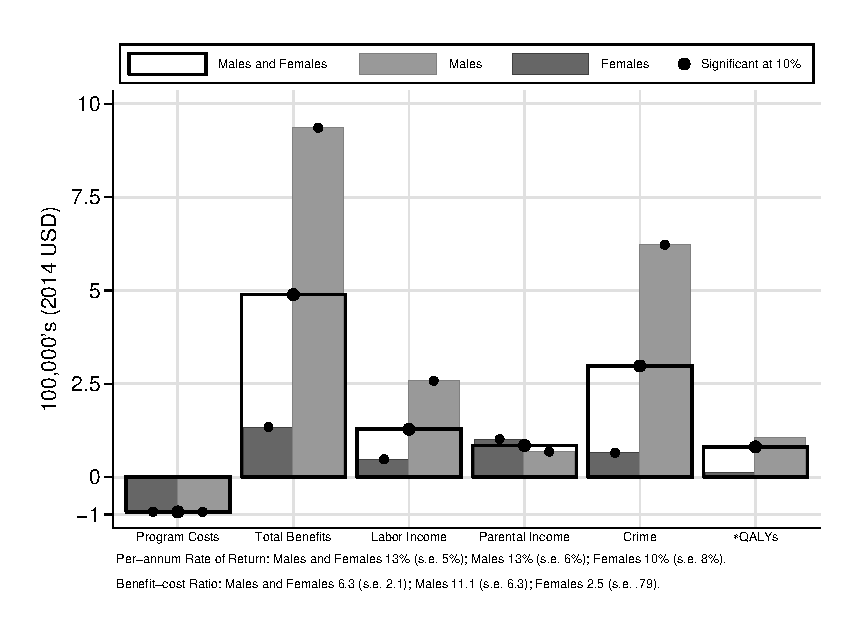
\includegraphics[width=.7\columnwidth]{output/abccare_npvssumm.eps}
\floatfoot{
\footnotesize
Note: This figure displays the life-cycle net present values of the main components of the cost/benefit analysis of ABC/CARE from birth to age 79, discounted to birth at a rate of 3\%.  By ``net" we mean that each component represents the total value for the treatment group minus the total value for the control group. Program costs: the total cost of implementing ABC/CARE. Total net benefits: the total net benefits of \textit{all} the components we consider. Labor income: total individual labor income from ages 20 to the retirement of program participants (assumed to be age 67). Parental income: total parental labor income of the parents icipants from when the participants were ages 1.5 to 21. Crime: the total cost of crime (judicial and victimization costs). Total medical costs: both private and public medical costs from ages 15 to 79. Costs of education: the total costs of education of the individual from ages 6 to 26 and include any costs from special education and grade retention. Inference is based on non-parametric, one-sided $p$-values from the empirical bootstrap distribution. We highlight point estimates significant at the $10\%$ level.\\
*QALYs refers to the quality-adjusted life years. Any gain corresponds to better health conditions through age 79.}
\end{sidewaysfigure}

The rest of the paper justifies and interprets these estimates. We proceed in the following way. Section~\ref{section:background} discusses main features of ABC/CARE. Section~\ref{section:methodsquestions} defines the parameters of interest.

Section~\ref{section:methodology} discusses our approaches to inference for vectors of treatment effects. We use  combining functions that summarize the \emph{number} of beneficial outcomes (as well as the number of statistically significant beneficial outcomes) within blocks of outcomes and overall. Section~\ref{section:c-functions} presents inference for combining functions. It also summarizes standard treatment effects of ABC/CARE. We account for multiple hypothesis testing by adjusting $p$-values for the multiplicity of reported outcomes to avoid cherry-picking ``significant'' results.\footnote{\citet{Lehman_Romano_2005_AnnStat,Romano_Shaikh_2006_AnnStat}. For an application, see, e.g., \cite{Heckman_Moon_etal_2010_QE}.}

Our main approaches for summarizing the multiple program treatment effects are benefit/cost and rate of return analyses. They provide economically interpretable summaries of the program and its components. Section~\ref{section:cbamethodology} discusses our method for predicting life-cycle outcomes to conduct the benefit/cost analyses. Section~\ref{section:cbaresults} presents and analyzes estimates of the benefit/cost ratios and rates of return.

Section~\ref{section:conclusion} summarizes the paper. There are substantial benefits that differ by gender. In terms of treatment effects, females benefit across more domains. However, the monetized value of the treatment effects is substantially greater for males. This discrepancy is largely driven by labor income and health benefits, as well as reduced crime for males.

\section[Background and Data Sources]{Background and Data Sources} \label{section:background}

\subsection{Overview}

ABC/CARE targeted disadvantaged children in Chapel Hill/Durham, North Carolina.\footnote{Both ABC and CARE were designed and implemented by researchers at the Frank Porter Graham Center of the University of North Carolina in Chapel Hill.} Table~\ref{tab:programcomparison} presents an overview and compares the two programs. Appendix~\ref{appendix:background} describes these programs in detail. Here, we summarize its main features.

The goals of the program are to enhance the early-life skills of a disadvantaged population. The program (i) supports language, motor, and cognitive development; (ii) minimizes high-risk behaviors; and (iii) develops socio-emotional competencies considered crucial for school success including task-orientation, competence in communications, independence, and pro-social behavior.\footnote{\citet{Ramey_Collier_etal_1976_CarolinaAbecedarianProject, Ramey_etal_1985_Project-CARE_TiECSE, Sparling_1974_Synth_Edu_Infant_SPEECH, Wasik_Ramey_etal_1990_CD, Ramey-etal_2012-ABC}.}

The program provides individualized treatment. Each child's progress is recorded and learning activities are appropriately adjusted every 2 to 3 weeks. Environments are organized to promote pre-literacy and access to a rich set of learning tools.\footnote{The ``Learningames'' approach was implemented by infant and toddler caregivers in 1:1 child-adult interactions. Each ``Learningames'' activity stated a developmentally-appropriate objective, the necessary materials, directions for teacher behavior, and expected child outcome.} The curriculum emphasizes active learning experiences, dramatic play, and basic ideas of order and category (``pre-academic skills''), as well as discipline and the ability to interact with and respect others.  At later ages (3 through 5), the program becomes increasingly structured, focusing on the development of ``socio-linguistic and communicative competence.''\footnote{\citet{Ramey-et-al_1977_Intro-to-ABC, Haskins_1985_CD, Ramey_1981_Modification, Ramey_Campbell_1979_SR, Ramey_Smith_1977_AJMD, Ramey_McGinness_etal_1982_Abecedarianapproach, Sparling_Lewis_1979_BOOKLearninggamesFirstThree,Sparling_Lewis_1984_BOOKLearningGamesThreesFours}.}

ABC recruited four cohorts of children born between 1972 and 1976. CARE recruited two cohorts of children, born in 1978 and 1979. The recruitment processes for each study were identical. Potential participant families were referred to researchers by local social service agencies and hospitals at the beginning of the mother's last trimester of pregnancy. Eligibility was determined by a score of 11 or above on a High-risk Index (HRI).\footnote{See Appendix~\ref{appendix:background} for details on the construction of the HRI. Maternal education, parental IQ, presence of the father, family income, and father's job stability are its major components.}

As shown in Table~\ref{tab:programcomparison}, the design and implementation of both ABC and CARE were similar. ABC had two phases, the first of which lasted from birth until age 5. In this phase, children were randomly assigned to either a treatment group that received center-based childcare or a control group. The second phase of treatment consisted of academic support from ages 5 through 8. CARE consisted of two treatment phases that were very similar to those of ABC. The first phase of CARE, also lasting from birth until age 5, contained an additional treatment arm, family education, designed to study the effects of improving home environments on child development.\footnote{\citet{Wasik_Ramey_etal_1990_CD}.}

Our analysis pools the treatment group in CARE that received the center-based ABC curriculum with the ABC treatment group. We do not use the data on the CARE treatment group that only received family education.\footnote{\citet{Campbell_Conti_etal_2014_EarlyChildhoodInvestments} and \citet{ABCCARE_Dataset} show that there is no effect of the CARE family education component alone.} We analyze the first stage of both programs (through age 5).\footnote{The second-phase treatment of ABC/CARE had very weak, if any, effects (for evidence, see \citealp{Campbell_Conti_etal_2014_EarlyChildhoodInvestments} and \citealp{ABCCARE_Dataset}). \citet{Campbell_Conti_etal_2014_EarlyChildhoodInvestments} establish the validity of pooling the data across the second arms of the experiments.}

\begin{table}[!htbp]
\centering
\caption{ABC and CARE, Program Comparison} \label{tab:programcomparison}
\begin{adjustbox}{max width=\textwidth}
\begin{threeparttable}
	\small
	\begin{tabular}{L{4cm} L{7cm} L{7cm} C{3cm}} \toprule
& \multicolumn{1}{c}{ABC}& \multicolumn{1}{c}{CARE} & \multicolumn{1}{c}{ABC = CARE ?} \\ \midrule
\textbf{Program Overview} &&\\
\hspace{.5cm} Years Implemented &1972--1982&1978--1985\\
\hspace{.5cm} First-phase & Birth to 5 years old & Birth to 5 years old &\checkmark \\
\hspace{.6cm} Treatment & & & \\
\hspace{.5cm} Second-phase & 5 to 8 years old & 5 to 8 years old &\checkmark \\
\hspace{.6cm} Treatment & & & \\
\hspace{.5cm} Recruited Sample &122&67\\
\hspace{.5cm} \# of Cohorts &4&2\\
\midrule
\textbf{Eligibility} & Socio-economic disadvantage according to a multi-factor index (see Section \ref{section:background})&Socio-economic disadvantage according to a multi-factor index (see Section \ref{section:background}) & \checkmark\\
 \midrule
\textbf{Control} &&\\
\hspace{.5cm} N &54&23\\
\hspace{.5cm} Compensation & Diapers from birth to age 3, unlimited formula from birth to 15 months & Diapers from birth to age 3, unlimited formula from birth to 15 months & \checkmark \\
\hspace{.5cm} Control   & \treatsubsabc & \treatsubscarec \\
\hspace{.6cm} Substitution & & \\
\midrule
\textbf{Treatment} & Center-based childcare & Center-based childcare and family education\\
\hspace{.5cm} \textbf{Center-based} \\
\hspace{.5cm} \textbf{Childcare} \\
\hspace{.5cm} N &53 (participated)&17\\
\hspace{.5cm} Intensity &6.5--9.75 hours a day for 50 weeks per year& 6.5--9.75 hours a day for 50 weeks per year & \checkmark\\
\hspace{.5cm} Components & Instruction, medical care, nutrition, social services & Instruction, medical care, nutrition, social services & \checkmark\\
\hspace{.5cm} Staff-to-child Ratio &1:3 during ages 0--1 &1:3 during ages 0--1 & \checkmark\\
&1:4--5 during age 1--4 &1:4--5 during age 1--4 & \checkmark\\
&1:5--6 during ages 4--5 & 1:5--6 during ages 4--5 & \checkmark\\
\hspace{.5cm} Staff Qualifications &Mixed diplomas; experienced& Mixed diplomas; experienced & \checkmark\\ \\
\hspace{.5cm} \textbf{Family Education}  & & \\
\hspace{.5cm} N & (not part of the program) &27\\
\hspace{.5cm} Intensity && Home visits lasting 1 hour. 2--3 per month during ages 0--3. 1--2 per month during ages 4--5\\
\hspace{.5cm} Curriculum & & Social and mental stimulation; parent-child interaction\\
\hspace{.5cm} Staff-to-child Ratio &&1:1\\
\hspace{.5cm} Staff Qualifications &&Home visitor training\\
\midrule
 \textbf{School-age Treatment} \\
 \hspace{.5cm} N& 46 (participated) &39\\
\hspace{.5cm} Intensity & Every other week& Every other week & \checkmark\\
\hspace{.5cm} Components & Parent-teacher meetings& Parent-teacher meetings & \checkmark\\
\hspace{.5cm} Curriculum & Reading and math &  Reading and math & \checkmark\\
\hspace{.5cm} Staff-to-child Ratio &1:1& 1:1 &\checkmark\\
\hspace{.5cm} Staff Qualifications &Graduate degree and training in special education & Graduate degree and training in special education & \checkmark\\
\bottomrule
\end{tabular}

\begin{tablenotes}
\small
\item Note: This table compares the main elements of ABC and CARE, summarized in this section. A \checkmark\ indicates that ABC and CARE had the same characteristic.
\end{tablenotes}
\end{threeparttable}
\end{adjustbox}
\end{table}

For both programs, from birth until the age of 8, data were collected annually on cognitive and socio-emotional skills, home environment, family structure, and family economic characteristics. After age 8, data on cognitive and socio-emotional skills, education, and family economic characteristics were collected at ages 12, 15, 21, and 30.\footnote{At age 30, measures of cognitive skills are unavailable for both ABC and CARE.} In addition, we have access to unique administrative criminal records and a full medical survey at age 34. This allows us to study the long-term effects of the programs along multiple dimensions of human development.\footnote{See Appendix~\ref{appendix:data} for a more comprehensive description of the data. In Appendix~\ref{appendix:randomization}, we document the balance in observed baseline characteristics across the treatment and control groups, once we drop the individuals for whom we have crime or health information, for which there is substantial attrition. Further, the methodology we propose addresses missing information in either of these two outcome categories.}

\subsection{Randomization Protocol and Compromises} \label{section:randomization}

Randomization for ABC/CARE was conducted at the family level. Pairs of siblings and twins were jointly randomized into either treatment or control groups.\footnote{Sibling pairs occurred when the two siblings were close enough in age such that both of them were eligible for the program.} Although we know that pairing was based on the HRI, maternal education, maternal age, and gender of the subject, we do not know the original pairs. ABC collected an initial sample of 122 subjects. 22 subjects did not complete the first-phase of treatment as initially assigned by the randomization. We characterize each of the cases in Appendix~\ref{appendix:background} and document that our estimates are robust when we adjust for missing data using standard methods.\footnote{In Appendix~\ref{appendix:assessingcc}, we compare the observed, baseline characteristics of the subjects in Table~\ref{table:abccompromises} to the observed, baseline characteristics of the subjects who complied to the initial treatment assignment. We find little evidence of differences.} We conduct a comparable analysis for the CARE sample.

\subsection{Control Group Substitution}

In ABC/CARE, many control group members attended alternative preschools.\footnote{See \cite{Heckman_Hohmann_etal_2000_QJE} on the issue of substitution bias in social experiments.} In ABC, \treatsubsabc\ of control-group subjects were enrolled in one of 11 local center-based childcare centers. In CARE, \treatsubscarec\ of the control group were enrolled in alternative preschools. Figure~\ref{fig:treatsubcare} shows (for each program) the cumulative distribution of the proportion of the first five years that control subjects were enrolled in alternative preschools. Figure~\ref{fig:treatsubcare_2} shows the proportion of the sample enrolled in an alternative school at a previous age who persist in an alternative at the indicated age. Figure~\ref{fig:proportion-alt-pre} shows the distribution of time spent in the alternative program for all control group participants. Figure~\ref{fig:salmonella} shows the enrollment of the control families into alternative preschool by age of child for the full sample, and for those who enrolled in any alternative preschool for however long. Enrollment increases with the age of children. Once enrolled, they stay enrolled, and children generally go for a full year.

Most of the alternative preschools received federal subsidies and were subject to federal regulations of the 1970 era.\footnote{Appendix~\ref{appendix:tetanus} discusses the federal standards of that day. See \citet{Department-of-Health_1968_DayCareRequirements,NCGA_1971_House-Bill-100,Ramey-et-al_1977_Intro-to-ABC,Ramey_Campbell_1979_SR,Ramey_McGinness_etal_1982_Abecedarianapproach, Burchinal_Campbell_etal_1997_CD}.} Child caregivers were required to be trained in early childhood education. The centers were required to implement an approved curricula designed to enhance cognitive, social, and linguistic competence in disadvantaged children.\footnote{\citet{Burchinal_etal_1989_CD_Daycare-Pre-K-Dev}.} The access of control-group children to alternative programs affects the interpretation of estimated treatment effects. We discuss this next.

\begin{sidewaysfigure}[!htbp]
\centering
\caption{Control Substitution Characteristics, ABC/CARE Control Group}\label{fig:control-sub}
\begin{subfigure}[h]{0.4\textwidth}
		\centering
		\caption{Enrollment} \label{fig:treatsubcare}
		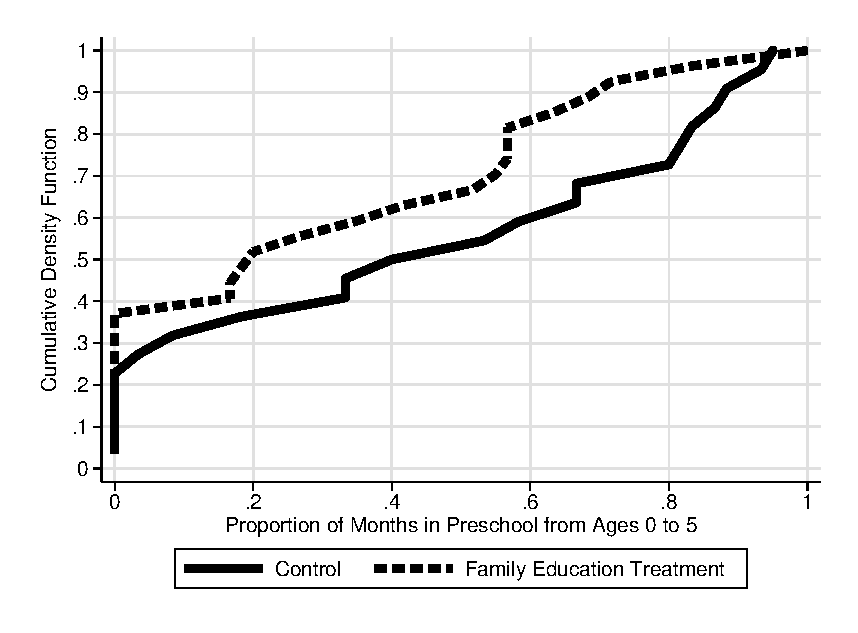
\includegraphics[width=\textwidth]{output/care_controlcontamination_months.eps}
\end{subfigure}%
\begin{subfigure}[h]{0.4\textwidth}
		\centering
		\caption{Enrollment Dynamics} \label{fig:treatsubcare_2}
		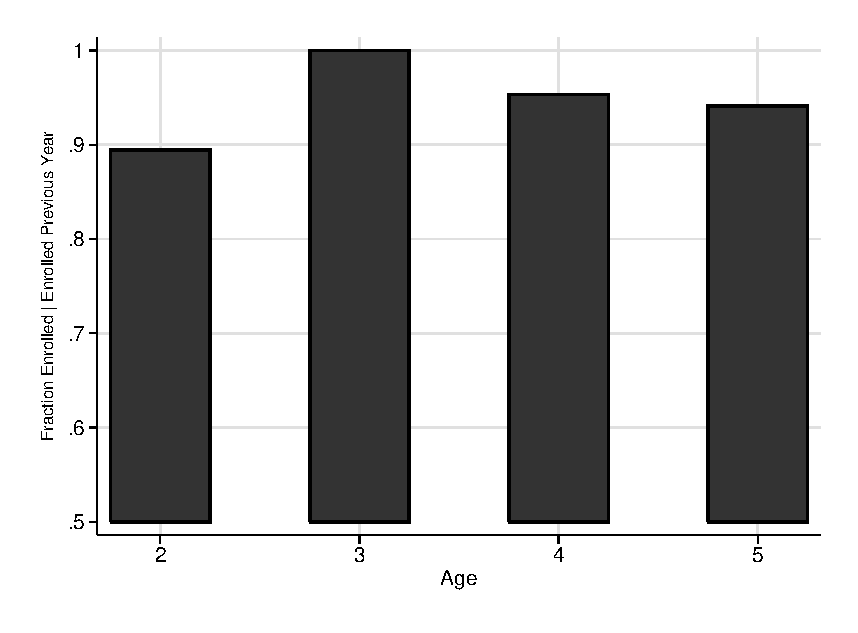
\includegraphics[width=\textwidth]{output/abccare_Vprobs.eps}
\end{subfigure}

\begin{subfigure}[h]{0.4\textwidth}
	\centering
	\caption{Enrollment Intensity} \label{fig:proportion-alt-pre}
		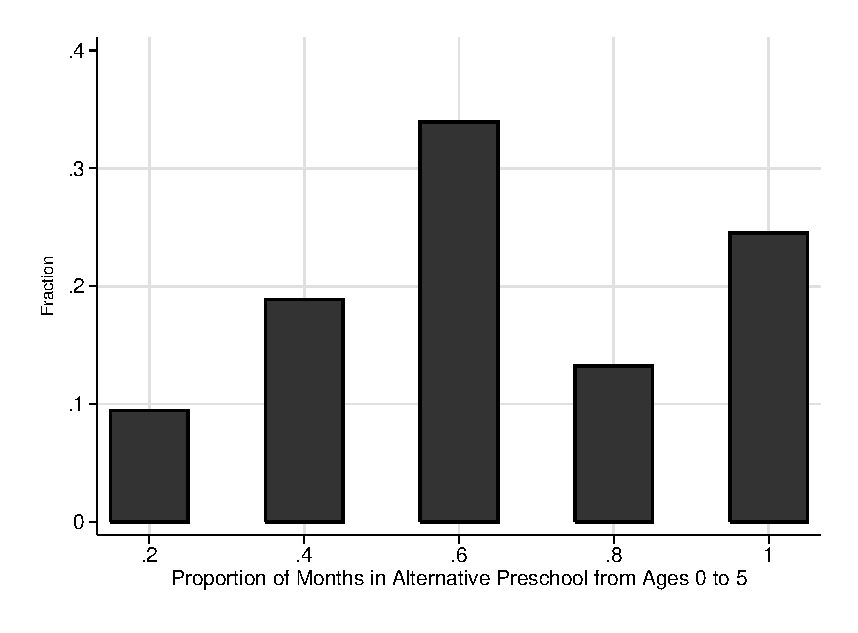
\includegraphics[width=\textwidth]{output/abccare_Vfractimes.eps}
\end{subfigure}%
\begin{subfigure}[h]{0.4\textwidth}
	\centering
	\caption{Enrollment by Age} \label{fig:salmonella}
		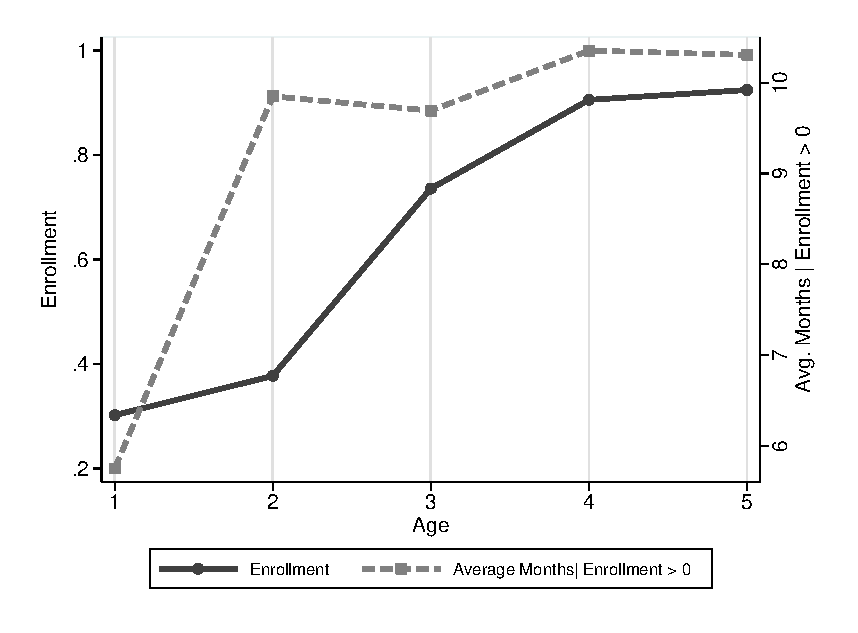
\includegraphics[width=\textwidth]{output/abccare_Valtenrollment.eps}
\end{subfigure}

\footnotesize \justify
Note: Panel (a) displays the cumulative distribution function of enrollment in alternative preschools of the ABC/CARE control group. Panel (b) displays the fraction of ABC/CARE control-group children enrolled in preschool, conditional on being enrolled in the previous age (at least one month). Panel (c) displays the fraction of children in the ABC/CARE control group enrolled in alternative preschools (fraction of children who were enrolled in alternative preschools 20\%, 40\%, 60\%, 80\%, and 100\% of the time, from ages 0 to 5). Panel (d) displays the fraction enrolled in alternative preschools of ABC/CARE control group by age in the left axis and average number of months in alternative preschool by age in the right axis. Both plots in Panel (d) are conditional on enrollment.\\
\end{sidewaysfigure}

\section{Parameters of Interest} \label{section:methodsquestions}

Random assignment to treatment does not guarantee that conventional treatment effects answer policy-relevant questions. We define and estimate three parameters that address different policy questions.

We assume that life cycles consist of $T+1$ discrete periods. The treatment phase is the first $\bar{t}$ periods of life $\left[0,\dots,\bar{t}\right]$. We have data up to age $t^{*}>\bar{t}$. We lack data on the remainder of life $(t^*,\dots,T]$. $W=1$ indicate that parents wish to participate in the program.\footnote{Individual subscripts are omitted to improve clarity.} $R \in \{0,1\}$ where $R=1$ indicates that a child is randomized into eligibility to participate in the program. Let $D$ indicate participation in the program.

Individuals are eligible to participate in the program if baseline background variables $\bm{B}\in\mathcal{B}_0$. In this paper, $\mathcal{B}_0$ is the set of scores on the high risk index (HRI) previously discussed. 

As it turns out, in the ABC/CARE study, all of the eligible persons ($\bm{B}\in\mathcal{B}_0$) given the option to participate choose to participate in the program $(W=1\text{, and } D=R)$. Thus, we can safely interpret the treatment effects generated by the experiment as average treatment effects for the population for which $\bm{B}\in\mathcal{B}_0$ and not just treatment effects for the treated (TOT). In Appendix~\ref{appendix:assessingcc}, we argue that, for all practical purposes, full compliance is a sensible assumption. There are few dropouts from the program. \emph{Ex ante} parents perceived that ABC/CARE was superior to other childcare alternatives.

Let $\bm{Y}^1_t$ be the outcome vector for the treated. $\bm{Y}^0_t$ is the outcome vector for those denied treatment in the program.

In principle, life-cycle treatment effects for the controls and treatment group members can depend on the exposures to treatment or to the various alternatives at each age. The pattern for controls is that most start in home care at the earliest ages and move to alternative preschools as the child ages (see Figure~\ref{fig:treatsubcare}). Once enrolled in an alternative preschool, they stay there through age 5 (see Figure~\ref{fig:treatsubcare_2}). It would be desirable to estimate treatment effects for each type of exposure but our samples are too small to make credible estimates for such detailed exposures. We simplify the analysis by creating two categories of control status. ``H'' denotes that the child is in home care throughout the entire length of the program. ``C'' denotes that the child was in an alternative preschool anytime. We test different categorizations in our empirical analysis reported below.

We thus compress a complex reality into two counterfactual outcome states at age $t$ for control group members:
\begin{align*}
\bm{Y}_{t,H}^0 \quad &: \quad \textbf{ Subject received home care exclusively} \\
\bm{Y}_{t,C}^0 \quad &: \quad \textbf{ Subject received some alternative childcare}.
\end{align*}

We define $V$ as a dummy variable indicating participation by controls in an alternative preschool. $V=0$ denotes staying at home. The counterfactual outcome when a child is in control status is $\bm{Y}^0_t$:
\begin{equation}
\bm{Y}^0_t : = \left( 1 - V \right) \bm{Y}^0_{t,H} + \left( V \right) \bm{Y}^0_{t,C}.
\end{equation}

One parameter of interest addresses the question: what is the effect of the program as implemented? This is the effect of the program compared to the next best alternative as perceived by the parents and is defined by
\begin{equation}\label{eq:effect}
\bm{\Delta}_t := \mathbb{E} \left[ \bm{Y}^1_t -  \bm{Y}^0_t | W =1 \right] := \mathbb{E} \left[\bm{Y}^1_t - \bm{Y}^0_t | \bm{B} \in \mathcal{B}_0 \right],
\end{equation}
where the second equality follows because everyone eligible wants to participate in the program. This parameter addresses the effectiveness of the program relative to the quality of all alternatives available when the program was implemented for the sample of eligible persons.

It is also fruitful to ask: what is the effectiveness of the program with respect to a counterfactual world in which the child stays at home full time? The associated causal parameter for those who would choose to keep the child at home is:
\begin{equation}\label{eq:influenza}
\bm{\Delta}_t \left(V = 0 \right) : =   \mathbb{E} \left[ \bm{Y}^1_t - \bm{Y}^0_t | V = 0, D = 1 \right] := \mathbb{E} \left[\bm{Y}^1_t - \bm{Y}^0_t | V = 0, \bm{B} \in \mathcal{B}_0 \right].
\end{equation}
Random assignment to the treatment group does not directly identify this parameter. The average effectiveness of a program relative to attendance in an alternative preschool for those who would choose an alternative is:
\begin{equation}\label{eq:smallpox}
\bm{\Delta}_t \left( V =1 \right) : =   \mathbb{E} \left[ \bm{Y}^1_t - \bm{Y}^0_t | V = 1, D = 1 \right] := \mathbb{E} \left[\bm{Y}^1 - \bm{Y}^0 | V = 1, \bm{B} \in \mathcal{B}_0 \right].
\end{equation}

\section{Summarizing Multiple Treatment Effects} \label{section:methodology}

ABC/CARE has rich longitudinal data on multiple outcomes over multiple periods of the life cycle. Summarizing these effects in an interpretable way is challenging. Appendix~\ref{appendix:results} presents step-down $p$-values for the blocks of outcomes that are used in our benefit/cost analysis which we summarize in this section.\footnote{\citet{Lehman_Romano_2005_AnnStat,Romano_Shaikh_2006_AnnStat}.}

Simpler, more digestible summary measures are useful for understanding the main empirical regularities in our data. This section discusses our approach to summarizing vectors of treatment effects using combining functions that count the proportion of treatment effects by category that show beneficial outcomes.

Consider a block of $N_l$ outcomes indexed by set $Q_l = \{1,\dots,N_l\}$. Let $j \in Q_l$ be a particular outcome within block $l$. Associated with it is a mean treatment effect
\begin{equation}
\Delta_{j,t} : = E(Y^1_{j,t} - Y^0_{j,t} | \bm{B} \in \mathcal{B}_0).
\end{equation}

We assume that outcomes can be ordered so that $\Delta_{j,t} >0$ is beneficial.\footnote{All but 5\% of the outcomes we study can be ranked in this fashion. See Appendix~\ref{appendix:results} for our classification.} We summarize the estimated effects of the program on outcomes within the block by the number of positive counts within block $l$:
\begin{equation}
C_l = \sum^{N_l}_{j=1} 1 (\hat{\Delta}_{j,t} >0).
\end{equation}
The proportion of beneficial outcomes in block $l$ is $C_l / N_l$.

Let $\mathcal{L}$ be the number of blocks. Under the null hypothesis of no treatment effects for all $j \in Q_l, l \in \mathcal{L}$, and assuming the validity of asymptotic approximations, $C_l / N_l$ should be centered around $1/2$. We bootstrap to obtain $p$-values for the null for each block and over all blocks. We also count the individually beneficial treatment effects that are statistically significant in the sets of outcomes across each of the groups indexed by the set $Q_l$. Using a 10\% significance level, on average 10\% of all outcomes should be ``significant'' at the 10\% level even if there is no treatment effect of the program. We provide evidence against both null hypotheses. 

Combing counts across all blocks enables us to avoid (i) arbitrarily picking outcomes that have statistically significant effects---``cherry picking''; or (ii) arbitrarily selecting blocks of outcomes to correct the $p$-values when accounting for multiple hypothesis testing.

\section{Empirical Estimates of Treatment Effects and Combining Functions}\label{section:c-functions}

ABC/CARE has hundreds of treatment effects corresponding to all of the measures collected in the multiple waves of the longitudinal surveys.\footnote{For estimates of treatment effects for each outcome analyzed, see Appendix~\ref{appendix:results}.} Reporting these treatment effects in the text would overwhelm the reader. Here we report estimates of the main treatment effects that underlie our benefit/cost and rate of return analyses.\footnote{Appendix~\ref{appendix:results} reports treatment effects and step-down $p$-values for all the outcomes analyzed. These account for multiple hypothesis testing as in \citet{Lehman_Romano_2005_AnnStat,Romano_Shaikh_2006_AnnStat}.}

Evidence from ABC/CARE and other early childhood programs is often criticized because of their small sample sizes.\footnote{See, e.g., \cite{Murray_2013_GivingKids_JJHBOOK}.} An extensive analysis reported in \citet{Campbell_Conti_etal_2014_EarlyChildhoodInvestments} shows that asymptotic inference and small sample permutation-based inference closely agree when applied to ABC/CARE data. For this reason, we use large sample inference throughout this paper.\footnote{Unless otherwise specified, the inference we present throughout the paper is based on $1,000$ draws from the empirical bootstrap distribution. $p$-values are one-sided, non-parametric. We high-light values when estimates are significant at $10\%$. For estimations using combining different datasets, we bootstrap all datasets and combine them to form bootstrap draws. Inference based on permutation tests is available on request.} We adjust all estimates for sample attrition using Horvitz--Thompson \citeyearpar{Horvitz_Thompson_1952_JASA} inverse probability estimators (see Appendix~\ref{appendix:attrition} for details). We account for control group substitution using a variety of econometric procedures: (a) matching, (b) instrumental variables, and (c) control functions. In the text, we rely on matching procedures to generate the inferences in this paper because the available instruments and exclusion restrictions are weak. Estimates from all of these procedures are in rough agreement, although the standard errors associated with IV and control function estimators are large. For further discussion, see Appendix~\ref{appendix:amethodology}.

\subsection{Treatment Effects}

The results for females show that the program increases employment, high school graduation, and college graduation and it reduces arrests (see Table~\ref{table:tescombined}). These results strengthen when we analyze females who did not receive alternative preschool. The results for education, child income, parental income, and crime are robust to controlling for substitution bias. The results for males are different. Treated subjects reported lower drug use and blood pressure. There are also effects on earnings and education. The results for employment, hypertension, blood pressure, and graduation from a 4-year college are strengthened when comparing the control group to those subjects who attend alternative preschools.

\newgeometry{top=.6in, bottom=.8in, left=.8in, right=.8in}
\begin{table}[!htbp]
\centering
\begin{threeparttable}
\caption{Treatment Effects on Selected Outcomes}\label{table:tescombined}
\begin{scriptsize}
  \begin{tabular}{ccccccccccc}
  \toprule
   Category & Variable & Age & (1) & (2) & (3) & (4) & (5) & (6)\\

    \midrule
     \multicolumn{9}{c}{\textbf{\emph{Females}}} \\ \\
    %cat 3
  \mc{1}{l}{\scriptsize{Parental Income}} &  \mc{1}{l}{\scriptsize{Parental Labor Income}} & \mc{1}{c}{\scriptsize{3.5}} & \mc{1}{c}{\scriptsize{2,756}} & \mc{1}{c}{\scriptsize{3,277}} & \mc{1}{c}{\scriptsize{10,509}} & \mc{1}{c}{\scriptsize{8,601}} & \mc{1}{c}{\scriptsize{-2,519}}  & \mc{1}{c}{\scriptsize{3,762}} \\  

  &   &  & \mc{1}{c}{\scriptsize{(0.206)}} & \mc{1}{c}{\scriptsize{(0.181)}} & \mc{1}{c}{\scriptsize{\textbf{(0.051)}}} & \mc{1}{c}{\scriptsize{\textbf{(0.058)}}} & \mc{1}{c}{\scriptsize{(0.614)}} & \mc{1}{c}{\scriptsize{(0.182)}} \\  

   &  & \mc{1}{c}{\scriptsize{12}} & \mc{1}{c}{\scriptsize{13,633}} & \mc{1}{c}{\scriptsize{19,386}} & \mc{1}{c}{\scriptsize{33,624}} & \mc{1}{c}{\scriptsize{26,474}} & \mc{1}{c}{\scriptsize{11,176}} & \mc{1}{c}{\scriptsize{18,629}} \\  

  &   &  & \mc{1}{c}{\scriptsize{\textbf{(0.061)}}} & \mc{1}{c}{\scriptsize{\textbf{(0.036)}}} & \mc{1}{c}{\scriptsize{(0.133)}} & \mc{1}{c}{\scriptsize{\textbf{(0.010)}}} & \mc{1}{c}{\scriptsize{(0.138)}} & \mc{1}{c}{\scriptsize{\textbf{(0.015)}}} \\  

 &    & \mc{1}{c}{\scriptsize{15}} & \mc{1}{c}{\scriptsize{8,565}} & \mc{1}{c}{\scriptsize{9,322}} & \mc{1}{c}{\scriptsize{5,533}} & \mc{1}{c}{\scriptsize{8,435}} & \mc{1}{c}{\scriptsize{8,817}} & \mc{1}{c}{\scriptsize{10,480}} \\  

  &   &  & \mc{1}{c}{\scriptsize{\textbf{(0.052)}}} & \mc{1}{c}{\scriptsize{\textbf{(0.090)}}} & \mc{1}{c}{\scriptsize{(0.354)}} & \mc{1}{c}{\scriptsize{(0.361)}} & \mc{1}{c}{\scriptsize{(0.114)}} & \mc{1}{c}{\scriptsize{\textbf{(0.058)}}} \\  

  &   & \mc{1}{c}{\scriptsize{21}} & \mc{1}{c}{\scriptsize{5,708}} & \mc{1}{c}{\scriptsize{6,944}} & \mc{1}{c}{\scriptsize{41,245}} & \mc{1}{c}{\scriptsize{25,135}} & \mc{1}{c}{\scriptsize{4,608}} & \mc{1}{c}{\scriptsize{3,926}} \\  

  &   &  & \mc{1}{c}{\scriptsize{(0.130)}} & \mc{1}{c}{\scriptsize{(0.214)}} & \mc{1}{c}{\scriptsize{\textbf{(0.023)}}} & \mc{1}{c}{\scriptsize{\textbf{(0.001)}}} & \mc{1}{c}{\scriptsize{(0.255)}} & \mc{1}{c}{\scriptsize{(0.265)}} \\  

 \mc{1}{l}{\scriptsize{Education}} &   \mc{1}{l}{\scriptsize{Graduated High School}} & \mc{1}{c}{\scriptsize{30}} & \mc{1}{c}{\scriptsize{0.253}} & \mc{1}{c}{\scriptsize{0.110}} & \mc{1}{c}{\scriptsize{0.561}} & \mc{1}{c}{\scriptsize{0.596}} & \mc{1}{c}{\scriptsize{-0.027}} & \mc{1}{c}{\scriptsize{0.066}} \\  

  &   &  & \mc{1}{c}{\scriptsize{\textbf{(0.012)}}} & \mc{1}{c}{\scriptsize{(0.208)}} & \mc{1}{c}{\scriptsize{\textbf{(0.001)}}} & \mc{1}{c}{\scriptsize{\textbf{(0.000)}}} & \mc{1}{c}{\scriptsize{(0.431)}} & \mc{1}{c}{\scriptsize{(0.310)}} \\  

  &  \mc{1}{l}{\scriptsize{Graduated 4-year College}} & \mc{1}{c}{\scriptsize{30}} & \mc{1}{c}{\scriptsize{0.134}} &  \mc{1}{c}{\scriptsize{0.119}}  & \mc{1}{c}{\scriptsize{0.112}} & \mc{1}{c}{\scriptsize{0.219}} & \mc{1}{c}{\scriptsize{0.095}} & \mc{1}{c}{\scriptsize{0.094}} \\  

  &   &  & \mc{1}{c}{\scriptsize{\textbf{(0.078)}}} &  \mc{1}{c}{\scriptsize{\textbf{(0.099)}}} & \mc{1}{c}{\scriptsize{(0.140)}} & \mc{1}{c}{\scriptsize{\textbf{(0.012)}}} & \mc{1}{c}{\scriptsize{(0.242)}} & \mc{1}{c}{\scriptsize{(0.210)}} \\  

  &  \mc{1}{l}{\scriptsize{Years of Education}} & \mc{1}{c}{\scriptsize{30}} & \mc{1}{c}{\scriptsize{2.143}} & \mc{1}{c}{\scriptsize{1.715}} & \mc{1}{c}{\scriptsize{3.370}} & \mc{1}{c}{\scriptsize{3.925}} & \mc{1}{c}{\scriptsize{1.238}} & \mc{1}{c}{\scriptsize{1.412}} \\  

  &   &  & \mc{1}{c}{\scriptsize{\textbf{(0.000)}}} & \mc{1}{c}{\scriptsize{\textbf{(0.007)}}} & \mc{1}{c}{\scriptsize{\textbf{(0.001)}}} & \mc{1}{c}{\scriptsize{\textbf{(0.000)}}} & \mc{1}{c}{\scriptsize{\textbf{(0.055)}}} & \mc{1}{c}{\scriptsize{\textbf{(0.023)}}} \\  

  \mc{1}{l}{\scriptsize{Labor Income}} &  \mc{1}{l}{\scriptsize{Employed}} & \mc{1}{c}{\scriptsize{30}} & \mc{1}{c}{\scriptsize{0.131}} & \mc{1}{c}{\scriptsize{0.079}} & \mc{1}{c}{\scriptsize{0.395}} & \mc{1}{c}{\scriptsize{0.340}} & \mc{1}{c}{\scriptsize{-0.004}} & \mc{1}{c}{\scriptsize{0.070}} \\  

 &    &  & \mc{1}{c}{\scriptsize{\textbf{(0.084)}}} & \mc{1}{c}{\scriptsize{(0.222)}} & \mc{1}{c}{\scriptsize{\textbf{(0.001)}}} & \mc{1}{c}{\scriptsize{\textbf{(0.037)}}} & \mc{1}{c}{\scriptsize{(0.483)}} & \mc{1}{c}{\scriptsize{(0.249)}} \\  

 &   \mc{1}{l}{\scriptsize{Labor Income}} & \mc{1}{c}{\scriptsize{30}} & \mc{1}{c}{\scriptsize{2,548}} & \mc{1}{c}{\scriptsize{2,412}} & \mc{1}{c}{\scriptsize{10,256}} & \mc{1}{c}{\scriptsize{14,862}} & \mc{1}{c}{\scriptsize{-1,078}} & \mc{1}{c}{\scriptsize{-822}} \\  

 &    &  & \mc{1}{c}{\scriptsize{(0.337)}} & \mc{1}{c}{\scriptsize{(0.363)}} & \mc{1}{c}{\scriptsize{(0.154)}} & \mc{1}{c}{\scriptsize{\textbf{(0.020)}}} & \mc{1}{c}{\scriptsize{(0.413)}} & \mc{1}{c}{\scriptsize{(0.457)}} \\  

  \mc{1}{l}{\scriptsize{Crime}} &  \mc{1}{l}{\scriptsize{Total Felony Arrests}} & \mc{1}{c}{\scriptsize{Mid-30s}} & \mc{1}{c}{\scriptsize{-0.328}} & \mc{1}{c}{\scriptsize{-0.394}} & \mc{1}{c}{\scriptsize{-1.006}} & \mc{1}{c}{\scriptsize{-0.965}} & \mc{1}{c}{\scriptsize{-0.083}} & \mc{1}{c}{\scriptsize{0.005}} \\  

   &  &  & \mc{1}{c}{\scriptsize{\textbf{(0.085)}}} & \mc{1}{c}{\scriptsize{\textbf{(0.078)}}} & \mc{1}{c}{\scriptsize{(0.119)}} & \mc{1}{c}{\scriptsize{\textbf{(0.096)}}} & \mc{1}{c}{\scriptsize{(0.237)}} & \mc{1}{c}{\scriptsize{(0.469)}} \\  

   & \mc{1}{l}{\scriptsize{Total Misdemeanor Arrests}} & \mc{1}{c}{\scriptsize{Mid-30s}} & \mc{1}{c}{\scriptsize{-0.973}} & \mc{1}{c}{\scriptsize{-1.212}} & \mc{1}{c}{\scriptsize{-2.303}} & \mc{1}{c}{\scriptsize{-2.448}} & \mc{1}{c}{\scriptsize{-0.466}} & \mc{1}{c}{\scriptsize{-0.201}} \\  

   &  &  & \mc{1}{c}{\scriptsize{\textbf{(0.055)}}} & \mc{1}{c}{\scriptsize{\textbf{(0.100)}}} & \mc{1}{c}{\scriptsize{(0.163)}} & \mc{1}{c}{\scriptsize{(0.125)}} & \mc{1}{c}{\scriptsize{(0.184)}} & \mc{1}{c}{\scriptsize{(0.297)}} \\  

  \mc{1}{l}{\scriptsize{Health}} &  \mc{1}{l}{\scriptsize{Self-reported drug user}} & \mc{1}{c}{\scriptsize{Mid-30s}} & \mc{1}{c}{\scriptsize{-0.033}} & \mc{1}{c}{\scriptsize{-0.039}} & \mc{1}{c}{\scriptsize{-0.221}} & \mc{1}{c}{\scriptsize{-0.101}} & \mc{1}{c}{\scriptsize{0.031}} & \mc{1}{c}{\scriptsize{0.033}} \\  

   &  &  & \mc{1}{c}{\scriptsize{(0.394)}} & \mc{1}{c}{\scriptsize{(0.382)}} & \mc{1}{c}{\scriptsize{(0.164)}} & \mc{1}{c}{\scriptsize{(0.300)}} & \mc{1}{c}{\scriptsize{(0.419)}} & \mc{1}{c}{\scriptsize{(0.401)}} \\  

  &  \mc{1}{l}{\scriptsize{Systolic Blood Pressure (mm Hg)}} & \mc{1}{c}{\scriptsize{Mid-30s}} & \mc{1}{c}{\scriptsize{-2.899}} & \mc{1}{c}{\scriptsize{-4.316}} & \mc{1}{c}{\scriptsize{-2.825}} & \mc{1}{c}{\scriptsize{-0.827}} & \mc{1}{c}{\scriptsize{-3.915}} & \mc{1}{c}{\scriptsize{-6.805}} \\  

  &   &  & \mc{1}{c}{\scriptsize{(0.311)}} & \mc{1}{c}{\scriptsize{(0.275)}} & \mc{1}{c}{\scriptsize{(0.438)}} & \mc{1}{c}{\scriptsize{(0.455)}} & \mc{1}{c}{\scriptsize{(0.320)}} & \mc{1}{c}{\scriptsize{(0.184)}} \\  

  &  \mc{1}{l}{\scriptsize{Diastolic Blood Pressure (mm Hg)}} & \mc{1}{c}{\scriptsize{Mid-30s}} & \mc{1}{c}{\scriptsize{-0.002}} & \mc{1}{c}{\scriptsize{1.323}} & \mc{1}{c}{\scriptsize{5.667}} & \mc{1}{c}{\scriptsize{4.120}} & \mc{1}{c}{\scriptsize{0.834}} & \mc{1}{c}{\scriptsize{-2.186}} \\  

  &   &  & \mc{1}{c}{\scriptsize{(0.485)}} & \mc{1}{c}{\scriptsize{(0.421)}} & \mc{1}{c}{\scriptsize{(0.265)}} & \mc{1}{c}{\scriptsize{(0.241)}} & \mc{1}{c}{\scriptsize{(0.445)}} & \mc{1}{c}{\scriptsize{(0.337)}} \\  

  &  \mc{1}{l}{\scriptsize{Hypertension}} & \mc{1}{c}{\scriptsize{Mid-30s}} & \mc{1}{c}{\scriptsize{0.172}} & \mc{1}{c}{\scriptsize{0.151}} & \mc{1}{c}{\scriptsize{0.112}} & \mc{1}{c}{\scriptsize{0.162}} & \mc{1}{c}{\scriptsize{0.177}} & \mc{1}{c}{\scriptsize{0.107}} \\  

  &   &  & \mc{1}{c}{\scriptsize{(0.112)}} & \mc{1}{c}{\scriptsize{(0.193)}} & \mc{1}{c}{\scriptsize{(0.312)}} & \mc{1}{c}{\scriptsize{(0.266)}} & \mc{1}{c}{\scriptsize{(0.188)}} & \mc{1}{c}{\scriptsize{(0.254)}} \\  

     
     
     
     
     
     
     
     
     
     
     
     
     
     
\midrule
    \multicolumn{9}{c}{\textbf{\emph{Males}}} \\ \\
    % cat 3
      \mc{1}{l}{\scriptsize{Parental Income}} &    \mc{1}{l}{\scriptsize{Parental Labor Income}} & \mc{1}{c}{\scriptsize{3.5}} & \mc{1}{c}{\scriptsize{1,036}} & \mc{1}{c}{\scriptsize{-1,185}} & \mc{1}{c}{\scriptsize{-2,321}} & \mc{1}{c}{\scriptsize{1,452}} & \mc{1}{c}{\scriptsize{-1,171}} & \mc{1}{c}{\scriptsize{703}} \\  

   &  &  & \mc{1}{c}{\scriptsize{(0.395)}} & \mc{1}{c}{\scriptsize{(0.348)}} & \mc{1}{c}{\scriptsize{(0.402)}} & \mc{1}{c}{\scriptsize{(0.412)}} & \mc{1}{c}{\scriptsize{(0.357)}} & \mc{1}{c}{\scriptsize{(0.425)}} \\  

   &  & \mc{1}{c}{\scriptsize{12}} & \mc{1}{c}{\scriptsize{7,085}} & \mc{1}{c}{\scriptsize{10,384}} & \mc{1}{c}{\scriptsize{20,007}} & \mc{1}{c}{\scriptsize{12,682}} & \mc{1}{c}{\scriptsize{7,791}} & \mc{1}{c}{\scriptsize{5,411}} \\  

   &  &  & \mc{1}{c}{\scriptsize{\textbf{(0.084)}}} & \mc{1}{c}{\scriptsize{\textbf{(0.034)}}} & \mc{1}{c}{\scriptsize{\textbf{(0.043)}}} & \mc{1}{c}{\scriptsize{\textbf{(0.079)}}} & \mc{1}{c}{\scriptsize{\textbf{(0.095)}}} & \mc{1}{c}{\scriptsize{(0.134)}} \\  

  &   & \mc{1}{c}{\scriptsize{15}} & \mc{1}{c}{\scriptsize{8,488}} & \mc{1}{c}{\scriptsize{7,185}} & \mc{1}{c}{\scriptsize{10,024}} & \mc{1}{c}{\scriptsize{4,915}} & \mc{1}{c}{\scriptsize{5,020}} & \mc{1}{c}{\scriptsize{4,379}} \\  

  &   &  & \mc{1}{c}{\scriptsize{\textbf{(0.090)}}} & \mc{1}{c}{\scriptsize{(0.130)}} & \mc{1}{c}{\scriptsize{(0.181)}} & \mc{1}{c}{\scriptsize{(0.292)}} & \mc{1}{c}{\scriptsize{(0.247)}} & \mc{1}{c}{\scriptsize{(0.297)}} \\  

  &   & \mc{1}{c}{\scriptsize{21}} & \mc{1}{c}{\scriptsize{12,732}} & \mc{1}{c}{\scriptsize{12,650}} & \mc{1}{c}{\scriptsize{-2,880}} & \mc{1}{c}{\scriptsize{-1,000}} & \mc{1}{c}{\scriptsize{17,027}} & \mc{1}{c}{\scriptsize{10,323}} \\  

  &   &  & \mc{1}{c}{\scriptsize{\textbf{(0.016)}}} & \mc{1}{c}{\scriptsize{\textbf{(0.064)}}} & \mc{1}{c}{\scriptsize{(0.500)}} & \mc{1}{c}{\scriptsize{(0.448)}} & \mc{1}{c}{\scriptsize{\textbf{(0.018)}}} & \mc{1}{c}{\scriptsize{\textbf{(0.043)}}} \\  

   \mc{1}{l}{\scriptsize{Education}} &    \mc{1}{l}{\scriptsize{Graduated High School}} & \mc{1}{c}{\scriptsize{30}} & \mc{1}{c}{\scriptsize{0.073}} & \mc{1}{c}{\scriptsize{0.130}} & \mc{1}{c}{\scriptsize{0.186}} & \mc{1}{c}{\scriptsize{0.084}} & \mc{1}{c}{\scriptsize{0.136}} & \mc{1}{c}{\scriptsize{0.063}} \\  

  &   &  & \mc{1}{c}{\scriptsize{(0.264)}} & \mc{1}{c}{\scriptsize{(0.164)}} & \mc{1}{c}{\scriptsize{(0.999)}} & \mc{1}{c}{\scriptsize{(0.334)}} & \mc{1}{c}{\scriptsize{(0.176)}} & \mc{1}{c}{\scriptsize{(0.326)}} \\  

  &  \mc{1}{l}{\scriptsize{Graduated 4-year College}} & \mc{1}{c}{\scriptsize{30}} & \mc{1}{c}{\scriptsize{0.170}} & \mc{1}{c}{\scriptsize{0.178}} & \mc{1}{c}{\scriptsize{0.347}} & \mc{1}{c}{\scriptsize{0.100}} & \mc{1}{c}{\scriptsize{0.167}} & \mc{1}{c}{\scriptsize{0.142}} \\  

  &   &  & \mc{1}{c}{\scriptsize{\textbf{(0.047)}}} & \mc{1}{c}{\scriptsize{(0.102)}} & \mc{1}{c}{\scriptsize{\textbf{(0.068)}}} & \mc{1}{c}{\scriptsize{(0.340)}} & \mc{1}{c}{\scriptsize{(0.134)}} & \mc{1}{c}{\scriptsize{(0.109)}} \\  

  &  \mc{1}{l}{\scriptsize{Years of Education}} & \mc{1}{c}{\scriptsize{30}} & \mc{1}{c}{\scriptsize{0.525}} & \mc{1}{c}{\scriptsize{0.785}} & \mc{1}{c}{\scriptsize{1.619}} & \mc{1}{c}{\scriptsize{0.782}} & \mc{1}{c}{\scriptsize{0.649}} & \mc{1}{c}{\scriptsize{0.343}} \\  

  &   &  & \mc{1}{c}{\scriptsize{(0.152)}} & \mc{1}{c}{\scriptsize{\textbf{(0.078)}}} & \mc{1}{c}{\scriptsize{(0.999)}} & \mc{1}{c}{\scriptsize{(0.150)}} & \mc{1}{c}{\scriptsize{(0.134)}} & \mc{1}{c}{\scriptsize{(0.254)}} \\  

    \mc{1}{l}{\scriptsize{Labor Income}} &   \mc{1}{l}{\scriptsize{Employed}} & \mc{1}{c}{\scriptsize{30}} & \mc{1}{c}{\scriptsize{0.119}} & \mc{1}{c}{\scriptsize{0.182}} & \mc{1}{c}{\scriptsize{0.048}} & \mc{1}{c}{\scriptsize{0.039}} & \mc{1}{c}{\scriptsize{0.231}} & \mc{1}{c}{\scriptsize{0.261}} \\  

   &  &  & \mc{1}{c}{\scriptsize{(0.126)}} & \mc{1}{c}{\scriptsize{\textbf{(0.032)}}} & \mc{1}{c}{\scriptsize{(0.999)}} & \mc{1}{c}{\scriptsize{(0.362)}} & \mc{1}{c}{\scriptsize{\textbf{(0.021)}}} & \mc{1}{c}{\scriptsize{\textbf{(0.012)}}} \\  

  &  \mc{1}{l}{\scriptsize{Labor Income}} & \mc{1}{c}{\scriptsize{30}} & \mc{1}{c}{\scriptsize{19,810}} & \mc{1}{c}{\scriptsize{27,373}} & \mc{1}{c}{\scriptsize{42,616}} & \mc{1}{c}{\scriptsize{23,950}} & \mc{1}{c}{\scriptsize{26,715}} & \mc{1}{c}{\scriptsize{21,068}} \\  

  &   &  & \mc{1}{c}{\scriptsize{\textbf{(0.093)}}} & \mc{1}{c}{\scriptsize{(0.151)}} & \mc{1}{c}{\scriptsize{(0.165)}} & \mc{1}{c}{\scriptsize{(0.111)}} & \mc{1}{c}{\scriptsize{(0.156)}} & \mc{1}{c}{\scriptsize{(0.139)}} \\  

   \mc{1}{l}{\scriptsize{Crime}} &    \mc{1}{l}{\scriptsize{Total Felony Arrests}} & \mc{1}{c}{\scriptsize{Mid-30s}} & \mc{1}{c}{\scriptsize{0.196}} & \mc{1}{c}{\scriptsize{0.392}} & \mc{1}{c}{\scriptsize{1.481}} & \mc{1}{c}{\scriptsize{1.338}} & \mc{1}{c}{\scriptsize{0.096}} & \mc{1}{c}{\scriptsize{0.184}} \\  

 &    &  & \mc{1}{c}{\scriptsize{(0.364)}} & \mc{1}{c}{\scriptsize{(0.319)}} & \mc{1}{c}{\scriptsize{(0.133)}} & \mc{1}{c}{\scriptsize{\textbf{(0.029)}}} & \mc{1}{c}{\scriptsize{(0.435)}} & \mc{1}{c}{\scriptsize{(0.409)}} \\  

 &   \mc{1}{l}{\scriptsize{Total Misdemeanor Arrests}} & \mc{1}{c}{\scriptsize{Mid-30s}} & \mc{1}{c}{\scriptsize{-0.501}} & \mc{1}{c}{\scriptsize{-0.243}} & \mc{1}{c}{\scriptsize{-0.193}} & \mc{1}{c}{\scriptsize{-0.033}} & \mc{1}{c}{\scriptsize{-0.276}} & \mc{1}{c}{\scriptsize{-0.508}} \\  

  &   &  & \mc{1}{c}{\scriptsize{(0.175)}} & \mc{1}{c}{\scriptsize{(0.349)}} & \mc{1}{c}{\scriptsize{(0.361)}} & \mc{1}{c}{\scriptsize{(0.439)}} & \mc{1}{c}{\scriptsize{(0.344)}} & \mc{1}{c}{\scriptsize{(0.178)}} \\  

     \mc{1}{l}{\scriptsize{Health}} &  \mc{1}{l}{\scriptsize{Self-reported drug user}} & \mc{1}{c}{\scriptsize{Mid-30s}} & \mc{1}{c}{\scriptsize{-0.333}} & \mc{1}{c}{\scriptsize{-0.398}} & \mc{1}{c}{\scriptsize{-0.693}} & \mc{1}{c}{\scriptsize{-0.557}} & \mc{1}{c}{\scriptsize{-0.309}} & \mc{1}{c}{\scriptsize{-0.330}} \\  

 &    &  & \mc{1}{c}{\scriptsize{\textbf{(0.024)}}} & \mc{1}{c}{\scriptsize{\textbf{(0.014)}}} & \mc{1}{c}{\scriptsize{\textbf{(0.001)}}} & \mc{1}{c}{\scriptsize{\textbf{(0.000)}}} & \mc{1}{c}{\scriptsize{\textbf{(0.058)}}} & \mc{1}{c}{\scriptsize{\textbf{(0.031)}}} \\  

  &  \mc{1}{l}{\scriptsize{Systolic Blood Pressure (mm Hg)}} & \mc{1}{c}{\scriptsize{Mid-30s}} & \mc{1}{c}{\scriptsize{-9.791}} & \mc{1}{c}{\scriptsize{-13.511}} & \mc{1}{c}{\scriptsize{19.304}} & \mc{1}{c}{\scriptsize{14.979}} & \mc{1}{c}{\scriptsize{-23.674}} & \mc{1}{c}{\scriptsize{-18.537}} \\  

  &   &  & \mc{1}{c}{\scriptsize{(0.112)}} & \mc{1}{c}{\scriptsize{\textbf{(0.074)}}} & \mc{1}{c}{\scriptsize{\textbf{(0.034)}}} & \mc{1}{c}{\scriptsize{\textbf{(0.000)}}} & \mc{1}{c}{\scriptsize{\textbf{(0.003)}}} & \mc{1}{c}{\scriptsize{\textbf{(0.019)}}} \\  

  &  \mc{1}{l}{\scriptsize{Diastolic Blood Pressure (mm Hg)}} & \mc{1}{c}{\scriptsize{Mid-30s}} & \mc{1}{c}{\scriptsize{-10.854}} & \mc{1}{c}{\scriptsize{-16.689}} & \mc{1}{c}{\scriptsize{-11.320}} & \mc{1}{c}{\scriptsize{-8.741}} & \mc{1}{c}{\scriptsize{-19.311}} & \mc{1}{c}{\scriptsize{-13.988}} \\  

  &   &  & \mc{1}{c}{\scriptsize{\textbf{(0.046)}}} & \mc{1}{c}{\scriptsize{\textbf{(0.000)}}} & \mc{1}{c}{\scriptsize{\textbf{(0.084)}}} & \mc{1}{c}{\scriptsize{\textbf{(0.020)}}} & \mc{1}{c}{\scriptsize{\textbf{(0.000)}}} & \mc{1}{c}{\scriptsize{\textbf{(0.018)}}} \\  

  &  \mc{1}{l}{\scriptsize{Hypertension}} & \mc{1}{c}{\scriptsize{Mid-30s}} & \mc{1}{c}{\scriptsize{-0.291}} & \mc{1}{c}{\scriptsize{-0.352}} & \mc{1}{c}{\scriptsize{0.020}} & \mc{1}{c}{\scriptsize{-0.075}} & \mc{1}{c}{\scriptsize{-0.470}} & \mc{1}{c}{\scriptsize{-0.435}} \\  

  &   &  & \mc{1}{c}{\scriptsize{\textbf{(0.039)}}} & \mc{1}{c}{\scriptsize{\textbf{(0.050)}}} & \mc{1}{c}{\scriptsize{(0.412)}} & \mc{1}{c}{\scriptsize{(0.371)}} & \mc{1}{c}{\scriptsize{\textbf{(0.012)}}} & \mc{1}{c}{\scriptsize{\textbf{(0.004)}}} \\  


     
     \bottomrule
    \end{tabular} 
\end{scriptsize}
\begin{tablenotes}
\tiny
Note: This table shows the treatment effects for categories outcomes that are important for our benefit/cost analysis. Systolic and diastolic blood pressure are measured in terms of mm Hg. Each column present estimates for the following parameters: \textbf{(1)} $\mathbb{E} \big[ \bm{Y}^1 - \bm{Y}^0 | D = 1]$; {\textbf{(2)} $\mathbb{E} \big[ \bm{Y}^1 - \bm{Y}^0 | \bm{B}, D=1 \big]$}; {\textbf{(3)} $\mathbb{E} \big[ \bm{Y}^1_t | \bm{B}, D=1 \big] - \mathbb{E} \big[ \bm{Y}^0_t | \bm{B}, V=0, D=0 \big]$}; {\textbf{(4)} $\mathbb{E} \big[ \bm{Y}^1 - \bm{Y}^0 | \bm{B}, V=0, D = 1 \big] $}; {\textbf{(5)} $\mathbb{E} \big[ \bm{Y}^1_t | \bm{B}, D=1 \big] - \mathbb{E} \big[ \bm{Y}^0_t | \bm{B}, V=1, D = 0 \big]$}; {\textbf{(6)} $\mathbb{E} \big[ \bm{Y}^1 - \bm{Y}^0 | \bm{B}, V=1 , D = 1\big]$}. We account for the following background variables ($\bm{B}$): Apgar scores at minutes 1 and 5 and the high-risk index. We define the high-risk index in Appendix~\ref{appendix:background} and explain how we choose the control variables in Appendix~\ref{appendix:bvariables}. Inference is based on non-parametric, one-sided $p$-values from the empirical bootstrap distribution. We highlight point estimates significant at the $10\%$ level.
\end{tablenotes}
\end{threeparttable}
\end{table}
\restoregeometry
\doublespacing

\subsection{Estimated Combining Functions}

We next report estimates of the proportion of beneficial effects by block and overall.\footnote{We consider a total of 95 outcomes that we classify in Appendix~\ref{appendix:results}. These are the outcomes that most clearly relate to the treatment offered by the program.} The analysis is based on treatment effect \eqref{eq:effect}. Figure~\ref{fig:ppositive} displays the results from this analysis: ABC/CARE positively impacted a large percentage of the outcomes. We show the counts for treatment compared to the next best alternative parents chose in Figure~\ref{fig:ppositivenb}. Proportionately more outcomes are beneficial for girls, but the proportions are high for both groups and well above the benchmark of 1/2. In Tables~\ref{table:abccare_rslt_pooled_counts} to \ref{table:abccare_rslt_female_counts_n10a10} of Appendix~\ref{appendix:results}, we show that a large and precise fraction of effects are positive for both genders for categories of outcomes spanning the life cycle, including a wide variety of health categories.

Using an $\alpha$-level of significance, one would expect to find that $\alpha\%$ of the treatment effects are statistically significant just from the operation of chance. For a 10\% level of significance, $46\%$ are statistically significant for females and $28\%$ for males (see Figure~\ref{fig:ppositive10}).

Figures~\ref{fig:ppositivehome} and Figure~\ref{fig:ppositivealternative} adjust the count in Figure~\ref{fig:ppositivenb} to analyze more clearly defined counterfactuals, treatment compared to stay at home and treatment compared to alternative preschool. This comparison indicates that females and males benefit differently from this treatment. Females benefit more from any treatment compared to staying at home while males benefit more from treatment compared to attending an alternative preschool, but not compared to staying at home. This pattern recurs throughout the paper. Boys benefit much less from alternative preschools than girls.

\begin{sidewaysfigure}[!htbp]
\centering
\caption{Positively Impacted Outcomes, ABC/CARE Males and Females}\label{fig:ppositive}
\begin{subfigure}[h]{0.4\textwidth}
		\centering
		\caption{Treatment vs. Next Best} \label{fig:ppositivenb}
		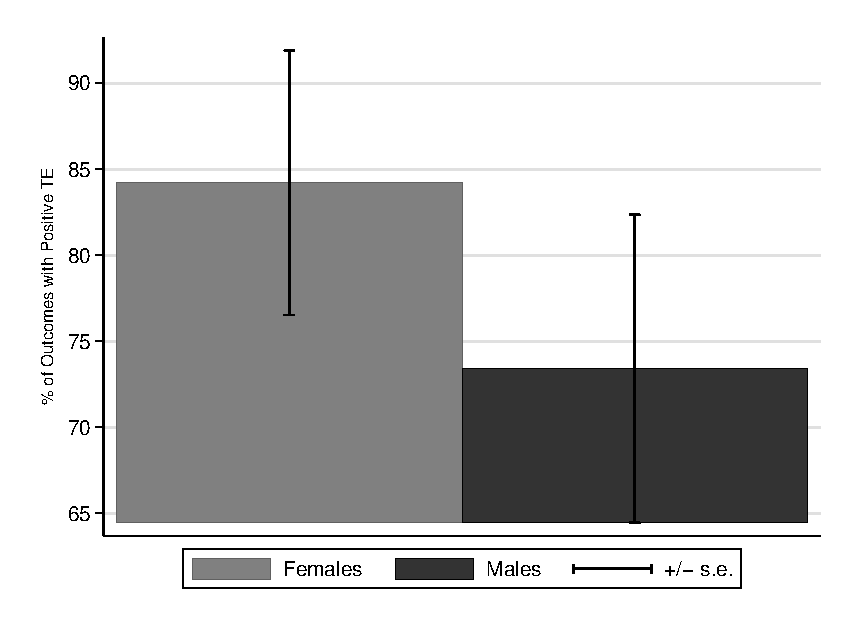
\includegraphics[width=\textwidth]{output/itt_noctrl_all.eps}
\end{subfigure}%
\begin{subfigure}[h]{0.4\textwidth}
	\centering
	\caption{Treatment vs. Next Best, Significant at 10\% Level} \label{fig:ppositive10}
		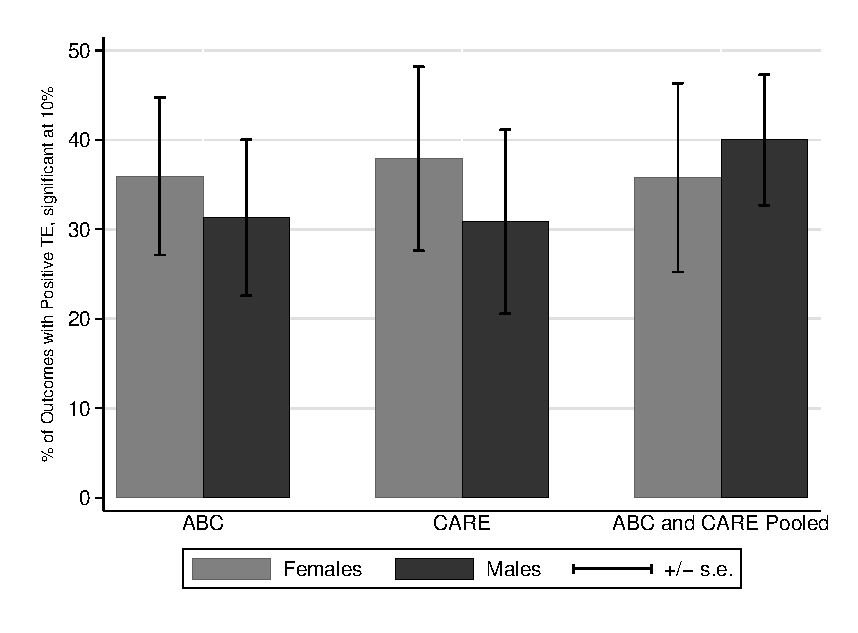
\includegraphics[width=\textwidth]{output/itt_noctrl_all_sig10.eps}
\end{subfigure}
\begin{subfigure}[h]{0.4\textwidth}
		\centering
		\caption{ Treatment vs. Stay at Home} \label{fig:ppositivehome}
		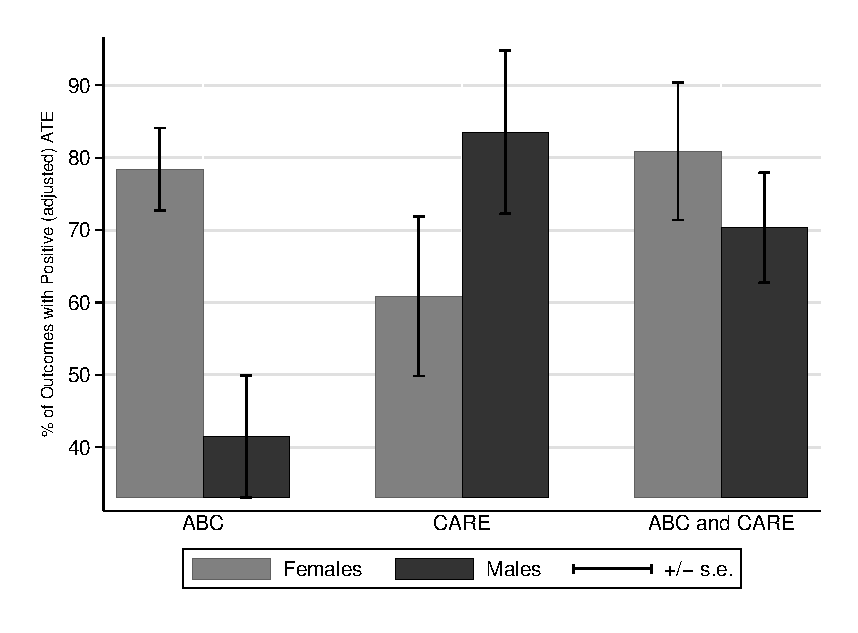
\includegraphics[width=\textwidth]{output/epan_ipw_p0_all.eps}
\end{subfigure}%
\begin{subfigure}[h]{0.4\textwidth}
	\centering
	\caption{Treatment vs. Alternative Preschool} \label{fig:ppositivealternative}
		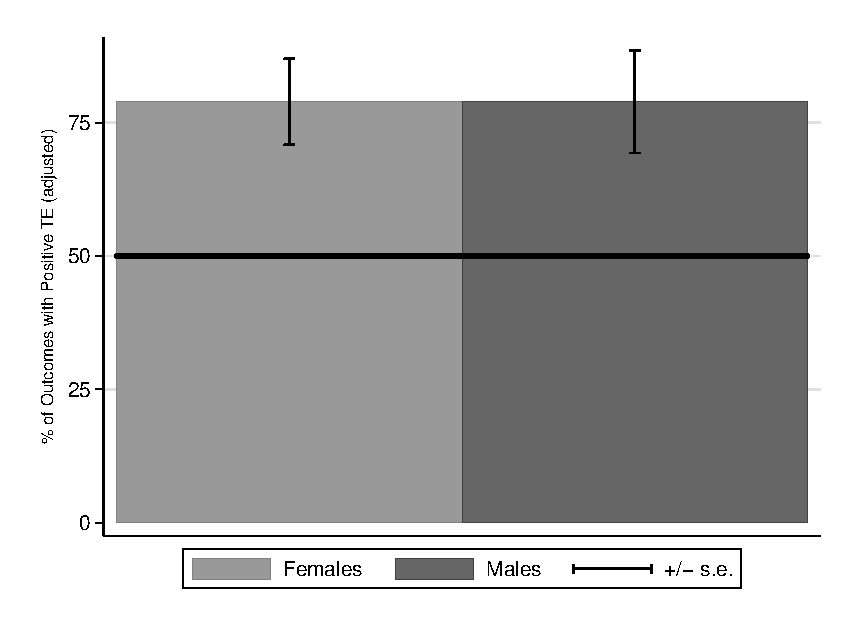
\includegraphics[width=\textwidth]{output/epan_ipw_p1_all.eps}
\end{subfigure}
\footnotesize \justify
Note: Panel (a) percentage of outcomes displaying a positive treatment effect, comparing treatment to next best. Panel (b) percentage of outcomes displaying a positive and significant treatment effect (10\% significance level). Panel (c) percentage of outcomes displaying a positive treatment effect, comparing treatment to staying at home. Panel (d) percentage of outcomes displaying a positive treatment effect, comparing treatment to alternative preschool. Standard errors are based on the empirical bootstrap distribution. For Panel (b) we perform a ``double bootstrap'' procedure to first determine significant treatment effects at $10\%$ level and then calculate the standard error of the count.\\
\end{sidewaysfigure}


\section{Predicting and Monetizing Life-cycle Costs and Benefits}\label{section:cbamethodology}

A central focus of this paper is on summarizing the multiple benefits of ABC/CARE using benefit/cost and rate of return analysis. This requires predicting the out-of-sample benefits of the program over the remaining life cycle. This is a fundamental problem in social science and has been addressed in the literature in multiple ways.\footnote{See, e.g., \cite{Heckman_Lochner_ea_2006_HEE}. \citet{Heckman_Moon_etal_2010_RateofReturn} use a variety of methods to project future earnings in the Perry study. The various methods are in general agreement. They fit a variety of panel data earnings dynamics models and project future earnings with them.} This section explains our strategy for using multiple data sources to extrapolate the life-cycle costs and benefits of education, labor income, transfer income, crime, and health. Our approach is motivated by the analysis of \citet{Heckman_Pinto_etal_2013_PerryFactor}, who show that the effect of treatment on outcomes operates through its effects of inputs in a stable production function. Practical details arising in implementing our approach are discussed in Appendix~\ref{appendix:methodology}.

\subsection{Using Auxiliary Samples to Predict Out of Sample Earnings}\label{sec:necrosis}

We have data on treatments and controls through age $t^{\ast}$. We lack information on participant outcomes afterward. Yet, post-$t^{\ast}$ outcomes are required to construct counterfactual life-cycle profiles. The goal is to find counterparts to both treatment and control individuals in the auxiliary data on whom we have post-$t^{\ast}$ data.

Because the participants of ABC/CARE are now in their mid-40s, there is no post-40s information on the same cohort  in any data. We use a synthetic cohort approach in which adjusted outcomes of older cohorts are used to estimate the future outcomes of the ABC/CARE participants. This approach is standard in the human capital literature. However, cohort effects may induce substantial biases.

Following the procedure in \citet{Heckman_Ichimura_etal_1998_REStud}, we use matching to find synthetic cohort counterparts in the auxiliary samples for both treatment and control group members. We match on baseline variables $\bm{B}$, as well as variables caused by treatment (i.e., for which there are treatment effects) that predict future outcomes---e.g., education, IQ, etc.---through age $t^{\ast}$. We then fit life-cycle relationships for outcomes beyond $t^{\ast}$ for the synthetic treatment and control groups using the initial conditions from the treatment and control groups at age $t^{\ast}$. From these predictions, we construct the life-cycle profiles. 

Let $\bm{Y}^{d}_{i,t}$ be an outcome at time $t$ for an individual in treatment status. Measured predictors of the outcome are $\bm{X}^{d}_{i,t}$ and $\bm{B}_i$.\footnote{$\bm{B}$ is balanced across treatments and controls by randomization.} We determine the predictors using within experimental sample analyses. We then find counterparts in the synthetic cohort samples. Let $S \in \{ 0,1\}$ denote membership in the experimental sample $(S=1)$ or the auxiliary sample, $(S=0)$.

For individual $i$, find counterparts $j(i)$ such that
\begin{equation}\label{eq:ingrownnail}
\sum_{j(i)\in F_0} \left( \bm{X}^{d}_{i,t} - \bm{X}_{j(i),t} \right)^{\prime} {\left( \bm{\Sigma}^d\right)}^{-1} \left(\bm{X}^{d}_{i,t} - \bm{X}_{j(i),t} \right) < \epsilon \text{ for } \qquad d \in \ \{0,1\}, t \in \{0,\dots,T\}
\end{equation}

\noindent where $\epsilon$ is arbitrarily small. $j(i) \in F_0$, for $t \leq t^{\ast}$, where $F_0$ is the index set in the auxiliary sample and $\bm{\Sigma}^d$ is the covariance matrix of the $\bm{X}$ in the experimental sample group $d$. We construct synthetic cohort samples using the same auxiliary samples and weight using the inverse value of~\eqref{eq:ingrownnail}. We fit dynamic relationships in the synthetic cohort sample over the whole sample period. Using the dynamic relationships in the synthetic cohort sample and the initial conditions from the experimental sample, we predict future outcomes. For this approach to be effective, we require that the support of the auxiliary sample includes the support of the experimental sample, an assumption formalized in the next subsection.\footnote{Evidence on this assumption is in Appendix~\ref{appendix:methodology}. In practice, we use indicators for black and male, year of birth, and years of education and labor income at age 30 as matching variables. We explain how we pick these variables and provide a sensitivity analysis to this choice in Appendix~\ref{appendix:methodology}.}

When samples are restricted to satisfy $\bm{B} \in \mathcal{B}_0$, given the small scale of the ABC/CARE program and the asynchrony of the experimental and synthetic cohort samples, it is reasonable to assume (in the absence of cohort effects) the synthetic cohort is equivalent to the control group $(D=0)$. This means that a test of the validity of our matching procedure is to compare the dynamic relationships fit on the synthetic cohort (with $\bm{B} \in \mathcal{B}_0$) constructed using the matching metric~\eqref{eq:ingrownnail} with the dynamic relationships for both treatments and controls within sample. 

A second test compares the post--$t^*$ outcomes for the auxiliary sample alone (with $\bm{B} \in \mathcal{B}_0$) and the constructed synthetic cohort. Figure~\ref{fig:labor-income-profiles} displays a comparison of these profiles. For females, Figure~\ref{fig:labor-income-profilesa} displays the dynamics relationship for the control group. Figure~\ref{fig:labor-income-profilesb} displays the post--$t^*$ dynamics for the auxiliary sample alone (with $\bm{B} \in \mathcal{B}_0$) and the constructed experimental sample. Figures~\ref{fig:labor-income-profilesc} and Figure~\ref{fig:labor-income-profilesd} display an analogous exercise for males.

It is also useful to compare pre--$t^*$ observed characteristics for (i) individuals with $\bm{B} \in \mathcal{B}_0$; (ii) the synthetic cohorts constructed based on \eqref{eq:ingrownnail}; and (iii) control-group individuals. Comparing (i) and (ii) allows us to asses if samples restricted to $\bm{B} \in \mathcal{B}_0$ are a comparable synthetic cohort in the absence of treatment; comparing (ii) and (iii) allows us to assess the quality of the matching procedure. Table~\ref{table:comp} presents this exercise. 

Testing whether the synthetic cohort constructed for the treatment group is a valid comparison is more complex than the above tests. There is not direct argument as when we compare the synthetic control-group cohort to the cohort such that $\bm{B} \in \mathcal{B}_0$. The reason is that treatment experimentally shifts human capital at early stages. When matching the individuals in the non-experimental sample to the treatment-group individuals, we could very well be obtaining matches to individuals with relatively higher unobserved ability (generating a standard omitted-variable bias). We develop this further in Section~\ref{section:just}. One comparison we can make, however, is between the synthetic treatment group we produce and the treatment group pre--$t^*$. Table~\ref{table:comp} evidences similarities. 

Our matching is based on indicators for black and male indicators, year of birth, years of education and labor income at age 30. We include labor income at age 21 and body-mass index at age 34 in the samples in which it is available to assess the quality of the matching out the variables targeted by the matching procedure.\footnote{We omit black because the experimental sample is $99\%$ black and year of birth because, by construction, this variable does not help to assess the matching. The auxiliary samples include younger individuals. We include it as part of the match to obtain year of birth matches that are as close as possible to the experimental group.}

\newgeometry{top=.6in, bottom=.8in, left=.8in, right=.8in}
\begin{sidewaystable}[!htbp] 
\begin{threeparttable}
\caption{Matching ABC/CARE to Non-Experimental Samples}
\label{table:comp}
\centering
\footnotesize 
\begin{tabular}{ccccccccccc} \toprule
\multicolumn{5}{c}{\textbf{Control}} & \multicolumn{5}{c}{\textbf{Treatment}} \\
Male  & Education (30)  & Labor Income (21) & Labor Income (30)  & BMI (34) & Male  & Education (30)  & Labor Income (21) & Labor Income (30)  & BMI (34)  \\  \midrule
\multicolumn{10}{l}{\textit{\textbf{ABC/CARE}}} \\
\multicolumn{10}{l}{\textbf{Actual}} \\
    0.487 &    12.279 & 13,890.419 & 26,083.818 &    32.737 &     0.507 &    13.646 & 14,057.678 & 38,461.222 &    31.299 \\  
    (0.503) &     (2.265) & (12,603.333) & (26,747.451) &     (7.168) &     (0.503) &     (2.414) & (11,472.872) & (58,824.180) &     (6.363) \\  
\multicolumn{10}{l}{\textbf{Predicted}} \\
        &         &         & 28,967.969 &         &         &         &         & 40,593.992 &         \\  
        &         &         & (32,662.494) &         &         &         &         & (56,871.180) &         \\  
        \multicolumn{10}{l}{\textit{\textbf{Non-experimental Synthetic Cohorts}}} \\
\multicolumn{10}{l}{\textbf{PSID}} \\
    0.472 &    12.898 &    & 31,311.562 &    26.835 &     0.479 &    13.080 &    & 32,445.578 &    26.737 \\  
    (0.499) &     (1.985) &     & (96,894.465) &     (5.779) &     (0.500) &     (1.993) &      &  (101,000.001) &     (5.729) \\  
\multicolumn{10}{l}{\textbf{NLSY79}} \\
    0.431 &    12.997 &   & 22,211.332 &  &     0.386 &    13.282 &   & 22,732.107 &  \\  
    (0.495) &     (1.938) &   & (10,960.699) & &     (0.487) &     (2.026) &   & (11,474.550) &  \\  
    \multicolumn{10}{l}{\textbf{CNLSY}} \\  
    0.471 &    12.923 & 11,503.405 & 25,873.078 &    29.229 &     0.478  &  12.923 & 11,487.266 & 25,940.491 &    29.244 \\  
    (0.499) &     (2.038) & (11,050.349) & (21,668.840) &     (6.712) &     (0.499) &     (2.033) & (11,061.850) & (21,793.892) &     (6.732) \\ 
        \multicolumn{10}{l}{\textit{\textbf{Non-experimental Sample with $\bm{B} \in \mathcal{B}_{0}$}}} \\ 
\multicolumn{10}{l}{\textbf{PSID}}\\
    0.500 &    12.763 &     & 23,298.833 &    29.708 &         &         &         &         &         \\  
    (0.500) &     (1.860) &      & (21,565.480) &     6.543 &         &         &         &         &         \\  
\multicolumn{10}{l}{\textbf{NLSY79}} \\
    0.542 &    11.520 &  & 17,191.630 &  &         &         &         &         &         \\  
    (0.498) &     (1.081) &   & (11,392.587) &  &         &         &         &         &         \\
    \multicolumn{10}{l}{\textbf{CNLSY}} \\  
    0.441 &    12.701 &  9,211.158 & 21693.718 &    30.058 &         &         &         &         &         \\  
    (0.497) &     (2.050) & (10,289.319) & (21,971.340) &     (7.022) &         &         &         &         &         \\  \bottomrule \end{tabular}

\begin{tablenotes}
\footnotesize
\item Note: Each column displays the mean and standard deviation in parentheses of the variables labeled in the first row. Age in which the variables is measured is in parentheses. We use the matching procedure in this section to obtain the control and treatment synthetic cohorts. For this exercise, $\bm{B} \in \mathcal{B}_0$ is defined as being black with maternal education of 12 years or less. Cells missing indicate that variables are not available in the non-experimental. We also omit $\bm{B} \in \mathcal{B}_0$ in the treatment columns. Standard deviations are based on the empirical bootstrap distribution.
\end{tablenotes}
\end{threeparttable}
\end{sidewaystable}
\restoregeometry
\doublespacing

As seen in Table~\ref{table:comp}, the average predicted labor income is very similar to the average observed labor income in both treatment and control groups. In addition to this correspondence in the levels, there is correspondence in the differences. Comparing the predicted and observed income between the treatment and control groups reinforces the true strength of the prediction: both differences are close to $\$12,000$.

When these methods are applied to the auxiliary data discussed in Section~\ref{section:cbaresults} they are effective. Figure~\ref{fig:control-sub} shows the prediction of labor income by comparing the prediction in the ABC/CARE data with the life-cycle profile of disadvantaged individuals in the PSID. Our pattern of life-cycle labor income is typical for low-skilled workers. See, e.g., \cite{Blundell-etal_2015_J-Pub-E}.\footnote{Our prediction is based on indicator variables of being male and being black, mother's education, average PIAT scores from ages 5 to 7, years of education at age 30, body-mass index at 34, labor income at ages 21 and 30, and one-period lagged labor income. A justification for the use of these variables, evidence on their predictive power, a sensitivity analysis to using different prediction variables are in Appendix~\ref{appendix:methodology}.}

A benchmark comparison for the labor income predictions we produce is to follow \citet{Mincer_1974_schooling}. We take our estimates of income at age 30 and calculate a perpetuity with a 3\% interest rate to correspond with our predicted NPV. This is because the Mincer-type estimates do not account for any income increase beyond age 30. Table~\ref{tab:mincerpred} presents the results from this exercise.

\begin{table}[htbp]
\centering
\begin{threeparttable}
\caption{Mincer-type Predictions, Age 30}\label{tab:mincerpred}
\small
\begin{tabular}{cccccc}
\toprule
Age-30 & Age-30 & Age-30 & Age-30 & Life-cycle & $\bm{r^*}$ \\
Prediction & Perpetuity ($r=10\%$) & Perpetuity ($r=7\%$) & Perpetuity ($r=3\%$) & Prediction &\\
 \midrule
\multicolumn{6}{c}{\textbf{Females}} \\ \\
\multicolumn{6}{c}{\emph{Control}} \\
23.187 &   241.176 &   344.537  &   803.920 &  1,017.098  & 2.28\% \\
(3.967) &     (1.321) &     (1.887) &     (4.404)  &     (0.908) & \\ \\
\multicolumn{6}{c}{\emph{Treatment}} \\
26.342 &   270.195 &   385.993 &   900.650 &  1,254.068  & 2.21\% \\
(4.664) &     (1.464) &    (2.092) &    (4.881) &    (0.932) &\\
\midrule
\multicolumn{6}{c}{\textbf{Males}} \\ \\
\multicolumn{6}{c}{\emph{Control}} \\
30.312 &   306.700 &   438.144 &  1,022.335 &  1,325.943 & 2.29\%  \\
(5.698) &    (1.897) &    (2.710) &    (6.324) &    (0.883)  &\\ \\
\multicolumn{6}{c}{\emph{Treatment}} \\
42.829 &   507.322 &   724.746 &  1,691.075  &  2,032.159 & 2.11\% \\
(9.532) &     (1.597) &     (2.281) &     (5.322) &     (1.006) &\\
\bottomrule
\end{tabular}

\begin{tablenotes}
\footnotesize
\item Note: This table presents Mincer-type predictions \citep{Mincer_1974_schooling}. Prediction at 30: predicted labor income at age 30 based on the procedure in Section~\ref{sec:necrosis}. Perpetuity based on 30: Prediction at 30/.03. Predicted Life-cycle: life-cycle predicted net present value of income based on the procedure in Section~\ref{sec:necrosis}. All values are in 1,000s (2014 USD). Standard errors are in parentheses and are based on the empirical bootstrap distribution.
\end{tablenotes}
\end{threeparttable}
\end{table}

\subsection{Justifying the Matching Procedure} \label{section:just}

To examine the validity of the matching approach just presented, and to provide an analytical framework for the extrapolation presented in this paper, it is helpful to introduce some general notation. Recall that $Y^d_{j,t}$ is $j$ at time $t$ for a treated person $(d\in\{0,1\})$. To simplify the analysis in this subsection, we do not further partition the control group. We define determinants of outcomes---vector $\bm{X}^d_t$---that may themselves be the outcomes of treatment, and may also depend on lagged outcomes also affected by treatment. Outcome variables are generated by the following equation
\begin{equation}\label{eq:trenchfoot}
Y^d_{j,t} = \phi^d_{j,t} (\bm{X}^d_t, \bm{B}, \varepsilon^d_{j,t}), \quad d \in \{0,1\}, \quad \  j \in \mathcal{J}_t, t \in \{0,\dots,T\}
\end{equation}
where $\mathcal{J}_t$ is the index set of possible outcomes and $\varepsilon^d_{j,t}$ is a scalar unobserved determinant of $Y^d_{j,t}$. $\bm{Y}^d_{t-1}$ can be included among the $\bm{X}^d_{t}$. We fit first order Markov relationships for earnings, transfer income, and health in our empirical models. The equation of motion for determinant $k \in \mathcal{K}_t$ (the set of determinants at time $t$) is given by
\begin{equation}\label{eq:frostbite}
X^d_{k,t} = \gamma^d_{k,t} (\bm{X}^d_{t-1}, \bm{B}, \eta^d_{k,t}), \quad d \in \{0,1\}, \ k \in \mathcal{K}_t, t \in \{0,\dots,T\}
\end{equation}
where $\eta^d_{k,t}$ is an unobserved determinant of $X^d_{k,t}$. For now, the dependence among the $\varepsilon^d_{j,t}$ and the $\eta^d_{k,t}$ is left unspecified. The $X^d_{k,t}$ can be caused by treatment, as can $X^d_{k,t-1}$. Examples of $\bm{X}^d_t$ in our data are education, IQ, health, work experience, and crime. All are potential determinants of earnings.

We assume \emph{structural invariance} of \eqref{eq:trenchfoot} and \eqref{eq:frostbite}.\footnote{See, e.g., \citet{Frisch_1938_autonomy}, \citet{Haavelmo_1943_Econometrica,Haavelmo_1944_Econometrica}, \citet{Hurwicz_1962_structural}, and \citet{Heckman_Pinto_2015_EconometTheory}.} This means that however the arguments of \eqref{eq:trenchfoot} and \eqref{eq:frostbite} are determined, for the same numerical values of $(\bm{X}^d_t, \bm{B}, \varepsilon^d_t)$ and $(\bm{X}^d_{t-1}, \bm{B}, \eta^d_{j,t})$, we obtain the same values of $Y^d_{j,t}$.\footnote{Frisch called this notion ``autonomy.'' Much later work in statistics captures structural invariance as one aspect of ``SUTVA.'' See \citet{Holland_1986_JASA} and \citet{Heckman_2008_ISR}.} This is a fundamental property of invariant economic relationships used by economists since the time of \citet{Frisch_1938_autonomy}.

\begin{assumption}\label{ass:butts}
(Structural Invariance)\\
\begin{spacing}{1.5}
\noindent Fixing $\bm{X}^d_t = (\bm{x}_t, \bm{b},\bar{\varepsilon}_t)$, $y^d_{j,t} = \phi^d_{j,t} (\bm{x}_t, \bm{b},  \bar{\varepsilon}^d_{j,t}) \quad j \in \mathcal{J}_t, \quad t \in \{0,\ldots,T\}$ is the same value assumed by $Y^d_{j,t}$ when $\bm{X}^d_{t-1} = \bm{x}_t$, $\bm{B} = \bm{b}$, and $\varepsilon^d_{j,t} = \bar{\varepsilon}_{j,t}$, and fixing $X^d_{t-1} = (x_{t-1}, b, \bar{\eta}_t)$, $X^d_{k,t} = \gamma^d_{k,t} (x_{t-1}, b, \bar{\eta}_t) \quad k \in \mathcal{K}_t$ assumes the same value as assumed by $X^d_{k,t-1} = x_{t-1}$, $B = b$, and $\eta^d_t = \bar{\eta}_t, t \in \{0,\dots,T\}$.
\end{spacing}
\end{assumption}

Equations~\eqref{eq:trenchfoot} and \eqref{eq:frostbite} can be estimated in the sample period $(0,\ldots,t^{*})$. We do not observe data on the experimental sample after $t^{*}$. To predict outside the sample period, we access auxiliary data on older cohorts of individuals whose life-cycle equations of motion are governed by Equations~\eqref{eq:trenchfoot} and \eqref{eq:frostbite}. This presumes the absence of cohort effects. We discuss the validity of this assumption when we turn to our empirical estimates.

\begin{assumption}\label{ass:crotchrot}
\textbf{Absence of Cohort Effects}
\end{assumption}

Our auxiliary data do not have direct information on program participation. However, given the limited size of the experimental sample, and the fact that the auxiliary cohorts were not eligible to participate in the program, it is reasonable to assume that no one in the auxiliary sample is treated ($D=0$). This means that \eqref{eq:trenchfoot} and \eqref{eq:frostbite} for $d=0$ can be identified over the supports of the available samples in the post-sample period. This implies that we can identify the post-experimental outcomes for the ABC/CARE control group if the support of the auxiliary data includes the support of the experimental data.

Let $\bm{Y}_j = (\bm{Y}^1_j, \bm{Y}^0_j)$, $\bm{X}_l = (\bm{X}^1_l, \bm{X}^0_l)$, $\varepsilon_n = (\varepsilon^1_n, \varepsilon^0_n)$, and define $\bm{X}^s = (\bm{X}_0,\dots,\bm{X}_T)^s$, $\bm{B}^s$ $\bm{Y}^s = (\bm{Y}_0,\dots,\bm{Y}_T)^s$, $\bm{\varepsilon}^s = (\varepsilon_0,\dots,\varepsilon_{T})^s$ where $s$ denotes sample membership. We assume

\begin{assumption} \label{ass:contain}
\begin{equation*}
\sup(\bm{X}, \bm{Y}, \bm{B}, \varepsilon)^{s=1} \subseteq \sup (\bm{X}, \bm{Y}, \bm{B}, \varepsilon)^{s=0}.
\end{equation*}
\end{assumption}
In particular, we assume that the support of $\mathcal{B}_0$ is included in the auxiliary sample.

Predicting treatment group outcomes is a more challenging task. We do so by invoking the assumption that outcome equations \eqref{eq:trenchfoot} and \eqref{eq:frostbite} are the same across treatment and control regimes. Formally, we assume

\renewcommand\theassumption{A--\arabic{assumption}(a)}
\begin{assumption}\label{ass:eczema}
For any $\bm{X}^d_t, \bm{B}, \varepsilon^d_{j,t}$ in $\sup(\bm{X},\bm{Y},\bm{B})^{s=0}$,
\begin{equation*}
\phi^1_{j,t} (\bm{X}^d_t, \bm{B}, \varepsilon^d_{j,t}) = \phi^0_{j,t} (\bm{X}^d_t, \bm{B}, \varepsilon^d_{j,t}) \qquad j \in \mathcal J_t, \quad t \in \{0,\dots,T\},
\end{equation*}
\end{assumption}
i.e., treatment effects operate through inputs and not shifts in the input-output functions. This allows us to use post-$t^*$ relationships fit on the auxiliary samples to forecast post-$t^*$ outcomes of treatment group members. Evidence for the validity of this assumption in the context of early childhood programs is presented in \citet{Heckman_Pinto_etal_2013_PerryFactor} and \citet{Attanasio-etal_2015_NBER_Estimating-Production}. Appendix~\ref{app:invariance} displays evidence favoring this assumption using our experimental sample.

We make a corresponding assumption for the equation governing the evolution of inputs:
\addtocounter{assumption}{-1}
\renewcommand\theassumption{A--\arabic{assumption}(b)}
\begin{assumption}\label{ass:psoriasis}
Given $\bm{X}^d_{t-1}, \bm{B}, \eta^d_{l,t}$,
\begin{equation*}
\gamma^1_{j,t} (\bm{X}^d_{t-1}, \bm{B}, \eta^d_{t-1}) = \gamma^0_{j,t} (\bm{X}^d_{t-1}, \bm{B}, \eta^d_{t-1}) \qquad k \in \mathcal{K}_t, \quad t \in \{0,\dots,T\}.
\end{equation*}
\end{assumption}
We assume that the elements of $\varepsilon_t^s, s \in \{0,1\}$, are mutually independent:

\renewcommand\theassumption{A--\arabic{assumption}}
\begin{assumption}\label{ass:corns}
\begin{align*}
&\varepsilon^s_{j,t} \indep \varepsilon^s_{k,t^\prime} | \bm{X}^s, s \in \{0,1\}\\
&\text{for all } j, k, t^\prime, \text{ and } t, \text{ except for } j=k \text{ and } t^\prime = t,\\
&j \in \mathcal{J}_t, \quad k \in \mathcal{K}_t \quad t \in \{0,\dots,T\}.
\end{align*}
\end{assumption}

\begin{theorem}
Putting Assumptions~\ref{ass:butts}--\ref{ass:corns} together, we obtain full observability of $\bm{X}^d_t$, estimation on the matched samples based on \eqref{eq:ingrownnail} generates unbiased out of sample treatment effects. $\Box$
\end{theorem}

Our prediction is based on matching individuals in the non-experimental samples to the control-group individuals. In the non-experimental samples, however, the dependence between $\mathbf{X}_{t}$ and $\varepsilon_{t}$ is generally different from that dependence in the experimental sample. While the experiment randomly shifts inputs of the production function of the forecasted outcome, in the non-experimental individuals with relatively high educated individuals could come from a better background, be more motivated, etc. This would bias our prediction because it would align it with a trend that does not correspond to the unobserved characteristics of the experimental sample. 

One solution for this problem is to obtain a measure of the potentially problematic unobserved component in the non-experimental sample and condition on it when estimating \eqref{eq:trenchfoot}, which we use to predict out of sample (in the experimental data). Three or more measures in the non-experimental sample would allow us to identify the distribution of this unobserved components and condition on them \citet{Cunha_Heckman_ea_2005_oep,Cunha_Heckman_etal_2010_est_tech_cognoncog}. If the endogeneity issue evolves dynamically, we would need these measures in every period. \textbf{[JLG: I'm exploring this. But I'm afraid we are asking too much from the non-experimental samples. We are already using various measures of PIAT for the match.]}


\begin{sidewaysfigure}[!htbp]
\centering
\caption{Labor Income Profile, Predictions and Comparison to PSID}\label{fig:labor-income-profiles}
\begin{subfigure}[h]{0.4\textwidth}
		\centering
		\caption{Prediction for ABC/CARE Females} \label{fig:labor-income-profilesa}
		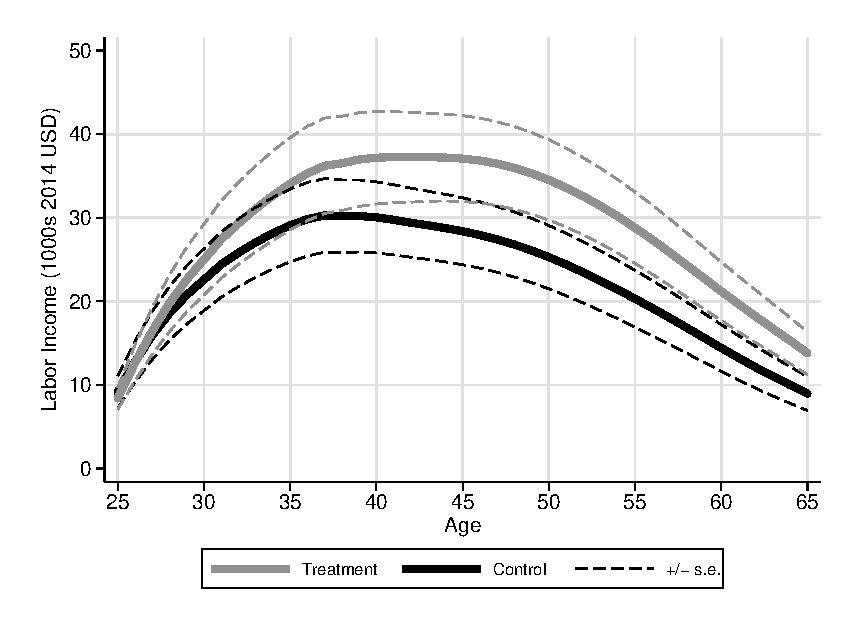
\includegraphics[width=\textwidth]{output/labor_25-65_pset1_mset3_female.eps}
\end{subfigure}%
\begin{subfigure}[h]{0.4\textwidth}
	\centering
	\caption{PSID, Disadvantaged Females} \label{fig:labor-income-profilesb}
		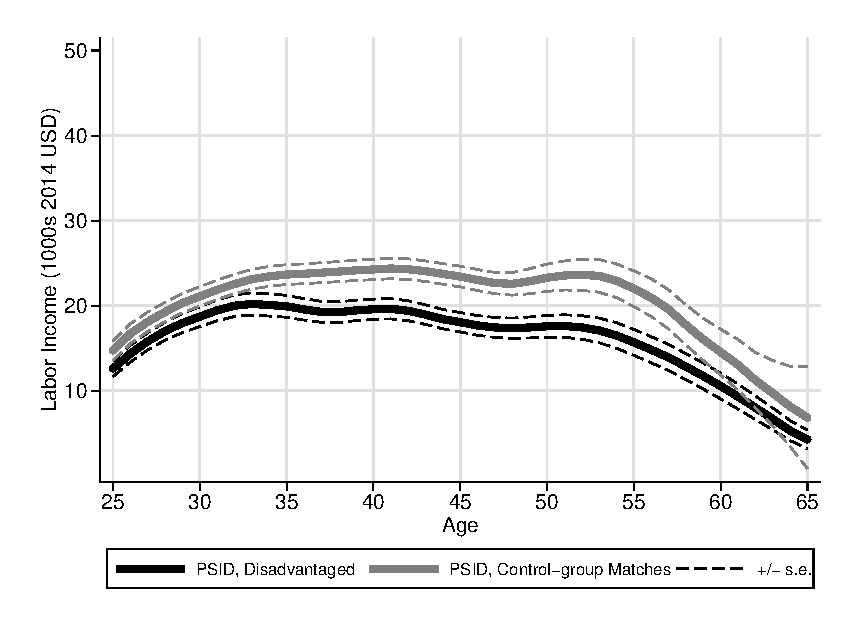
\includegraphics[width=\textwidth]{output/psid_B0_match_s0}
\end{subfigure}
\begin{subfigure}[h]{0.4\textwidth}
		\centering
		\caption{Prediction for ABC/CARE Males} \label{fig:labor-income-profilesc}
		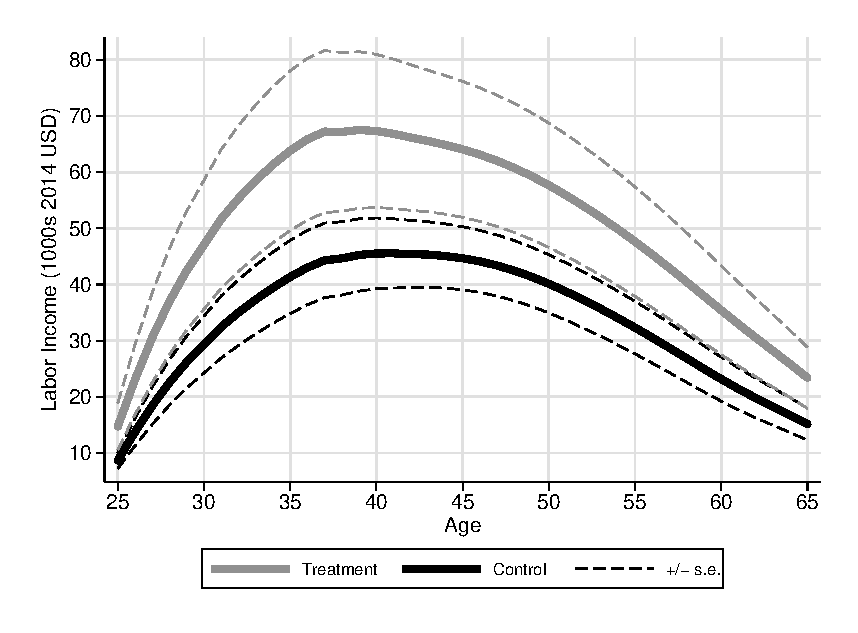
\includegraphics[width=\textwidth]{output/labor_25-65_pset1_mset3_male.eps}
\end{subfigure}%
\begin{subfigure}[h]{0.4\textwidth}
	\centering
	\caption{PSID, Disadvantaged Males} \label{fig:labor-income-profilesd}
		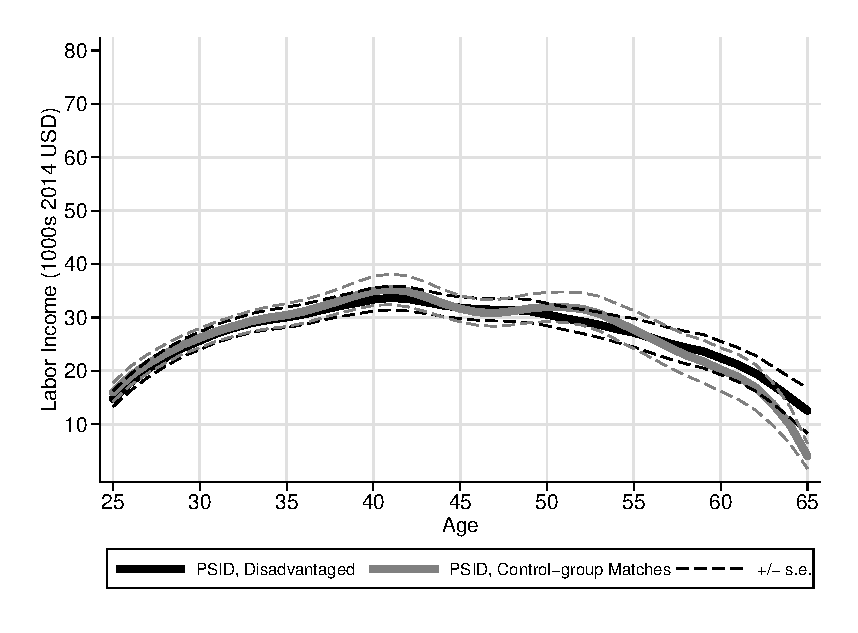
\includegraphics[width=\textwidth]{output/psid_B0_match_s1.eps}
\end{subfigure}
\footnotesize \justify
Note: Panels (a) and (c) display the predicted labor income profiles for ABC/CARE females and males by treatment status, based on predictions that combine data from the Panel Study of Income Dynamics (PSID), the National Longitudinal Survey of Youth 1979 (NLSY79), and the Children of the National Longitudinal Survey of Youth 1979 (CNLSY79). Panels (b) display the predicted labor income profiles of disadvantaged females ($\bm{B} \in \mathcal{B}_0$) in the PSID and control group matches in the PSID. The matches are constructed according to the procedure in Section~\ref{sec:necrosis}. For this exercise, we define disadvantaged females ($\bm{B} \in \mathcal{B}_0$) as black females whose mothers have 12 years of education or less. Panel (d) displays an analogous exercise for males. Standard errors are based on the empirical bootstrap distribution.\\
\end{sidewaysfigure}

\subsection{Health} \label{section:health}

To predict and monetize health outcomes requires an adaptation of the method we just explained. We consider three additional issues: (i) health outcomes such as diabetes or heart disease are absorbing states; (ii) health outcomes are highly interdependent within and across time periods; and (iii) there is no obvious terminal time period for benefits and costs except death, which is endogenous.\footnote{For example, for income we extrapolate up to the retirement age of 67. However, for health, we need to predict an age of death for each individual.} Our auxiliary model for health is an adaptation of the Future America Model (FAM). This model predicts health outcomes from the subjects' mid-30s up to their projected death \citep{Goldman_etal_2015_Future-Elderly-Model-Report}.\footnote{The simulation starts at the age in which we observe the subject's age-34 health follow-up. On average this happened at age 34 for both males and females, but there is variation ranging from age 30 to age 37.} Appendix~\ref{appendix:health} discusses the FAM methodology in detail. We initialize the health prediction using the same variables that we use when predicting labor and transfer income, along with the initial health conditions as listed in Table~\ref{table:transition}.

The methodology has five steps: (i) estimate age-by-age health state transition probabilities using the Panel Study of Income Dynamics (PSID); (ii) match these transition probabilities to the ABC/CARE subjects based on observed characteristics; (iii) estimate quality-adjusted life year (QALY) models using the Medical Expenditure Panel Survey (MEPS) and the PSID; (iv) estimate medical cost models using the MEPS and the Medicare Current Beneficiary Survey (MCBS), allowing estimates to differ by health state and observed characteristics; and (v) predict the medical expenditure and QALYs that correspond to the simulated individual health trajectories.\footnote{As an intermediate step between (i) and (ii), we impute some of the variables used to initialize the FAM models (see Appendix~\ref{appendix:health}).}

Our microsimulation model starts the health predictions at age 30, with the information on observed characteristics available at this age. Restricting it to the individuals for whom we have information from the age-34 health follow-up allows us to account for components that are crucial for predicting health outcomes, such as the body mass index (BMI) and measures of diastolic and systolic health. The models predict the probability of being in any of the states in the horizontal axis of Table~\ref{table:transition} at age $a+1$ based on the state at age $a$, which is described by the vertical axis of the table.\footnote{In practice, the predictions are based on two-year lags, due to data limitations in the auxiliary sources we use to simulate the FAM. For example, if the individual is 30 (31) years old in the age-30 interview, we simulate the trajectory of her health status at ages 30 (31), 32 (33), 34 (35), and so on until her projected death.} Absorbing states are an exception. For example, heart disease at age $a$ does not enter in the estimation of transitions for heart disease at age $a+1$ because it is an absorbing state: once a person has heart disease, she carries it through the rest of her life.

\begin{sidewaystable}[!htbp]
\begin{threeparttable}
\caption{Health State Transitions, Age $a$ as Predictor of Age $a+1$}\label{table:transition}
\scriptsize
\begin{tabular}{l|cccccccccccccc} \toprule
\multicolumn{1}{c}{Age $a$} & \multicolumn{14}{c}{Age $a+1$} \\ \midrule
  & Heart & Hyper- & Stroke & Lung  & Diabetes & Cancer & Disability & Mortality & Smoking  & Obesity & Health  & DI  & SS  & SSI  \\
&  Disease & tension &  & Disease & & & & &  &  & Insurance & Claim & Claim & Claim \\
Heart Disease & & & $\times$& & & &$\times$ &$\times$ & $\times$           &       &  $\times$  & $\times$ & $\times$ & $\times$\\
Hypertension  &  $\times$& & $\times$ & & & &$\times$ &$\times$ &       &     & $\times$   & $\times$ & $\times$  & $\times$\\
Stroke           & & & & & & &$\times$ &$\times$ &             &      &   $\times$  & $\times$ & $\times$  & $\times$\\
Lung Disease & & & & & & &$\times$ &$\times$ & $\times$         &        &   $\times$  &$\times$  & $\times$  & $\times$\\
Diabetes       & $\times$ &$\times$  & $\times$   & & & &$\times$ &$\times$ & $\times$            &       &  $\times$    & $\times$& $\times$ & $\times$ \\
Cancer         & & & $\times$ &  & &   &$\times$ & $\times$&           &         &   $\times$  & $\times$ & $\times$  & $\times$\\
Disability     & & & & & & &$\times$ &$\times$ &         &      &     $\times$  & $\times$ & $\times$   & $\times$\\
\midrule
Smoking & $\times$& $\times$&$\times$ & $\times$& $\times$& $\times$&$\times$ &$\times$ & $\times$   &   &     $\times$  & $\times$ & $\times$   & $\times$\\
BMI & $\times$& $\times$&$\times$ & $\times$& $\times$& $\times$&$\times$ & & $\times$    &  $\times$ &     &  &   & \\
Physical Activ. & $\times$& $\times$&$\times$ & $\times$& $\times$& $\times$&$\times$ & & $\times$    &   &     &   &  & \\
Binge Drinking & & & & & & &  &$\times$ & $\times$    &      &      &   &     &  \\
\midrule
DI Claim      & & & & &  & & & &             &         & $\times$    & $\times$   & $\times$ & $\times$\\
SS Claim     & & & & & & & &           &         &     & $\times$ &  & & $\times$\\
SSI Claim   & & & & &&  & & &         &        &      & &   & $\times$\\ \bottomrule
\end{tabular}

\begin{tablenotes}
\footnotesize
\item Note: This table illustrates how health outcomes at age $a$ predict health outcomes at age $a+1$. The crosses indicate if we use the age $a$ outcome to predict the age $a+1$ outcome. DI Claim: disability insurance claim; SS Claim: social security claim; DB Claim: disability benefits claim; SSI Claim: supplemental security income claim. The age $a$ states that do not predict themselves at age $a+1$ are absorbing states by construction.
\end{tablenotes}
\end{threeparttable}
\end{sidewaystable}

At each age, once we obtain the transition probability for each health outcome, we draw a Monte-Carlo simulation for each subject. Thus, each simulation depends on each individual's health history and on their particular characteristics. For every simulated trajectory of health outcomes, we predict the lifetime medical expenditure using the models estimated from the MEPS and the MCBS. We then obtain an estimate of the expected lifetime medical expenditure by taking the mean of each individual's simulated lifetime medical expenditure.

The same procedure is applied to calculate quality-adjusted life years (QALYs).\footnote{A quality-adjusted life year (QALY) reweighs a year of life according to its quality given the burden of disease. Suppose we assign a value of $\$150,000$ (2014 USD) to each years of life. A QALY of $\$150,000$ denotes a year of life in the absence of disease (perfect health). The value of QALY for an individual in a given year is smaller than $\$150,000$ when there is positive burden of disease, as worse health conditions imply lower QALYs. When an individual dies, her QALY equals zero. It is worth noting that there are extreme combinations of disease and disability that may generate negative QALYs, although this case is unusual.} We compute a QALY model based on the EQ-5D instrument, a widely-used Health-related Quality-of-life (HRQoL) measure, available in MEPS. We then estimate this model from the PSID.

We estimate three models of medical spending: (i) Medicare spending (annual medical spending paid by parts A, B, and D of Medicare); (ii) out-of-pocket spending (medical spending paid directly by the individual); and (ii) all public spending other than Medicare. Each medical spending model includes a individuals the variables we use to predict labor and transfer income, current health, risk factors, and functional status as explanatory variables. The MCBS-based medical spending models also include lagged health because of the length of time for which MCBS subjects are observed.

We also calculate medical expenditure before age 30. We combine the MEPS and retrospective information in the ABC/CARE interviews at ages 21 and 30 related to hospitalizations at ages 12 and 15 and births at age 15. In addition to this retrospective information, we use use individual and family demographics to predict medical expenditure models for each age.

The first level of each model predicts the likelihood that the subject incurred any medical expenditure in the period. The second level predicts the medical expenditure for those with positive expenditures.

QALYs are crucial to our estimations because they monetize the health of an individual at each age. Figure~\ref{fig:qalys} shows our estimation of QALYs together with a PSID comparison, in an analogous exercise to Figure~\ref{fig:labor-income-profiles}.\footnote{In our baseline estimation, we assume that each year of life is worth  $\$150,000$ (2014 USD). Our estimates are robust to substantial variation in this assumption, as we show in Appendix~\ref{appendix:sensitivity}.} Although there is not a clear age-by-age treatment effect on QALYs, there is a significant difference in the accumulated present value of the QALYs between the treatment and the control groups. The QALYs for individuals in the control group match the QALYs of low-skilled individuals in the PSID.

\begin{sidewaysfigure}[!htbp]
\centering
\caption{Quality Adjusted Life Years, Predictions and Comparison to PSID}\label{fig:qalys}
\begin{subfigure}[h]{0.5\textwidth}
		\centering
		\caption{Females} \label{fig:qabcare1}
		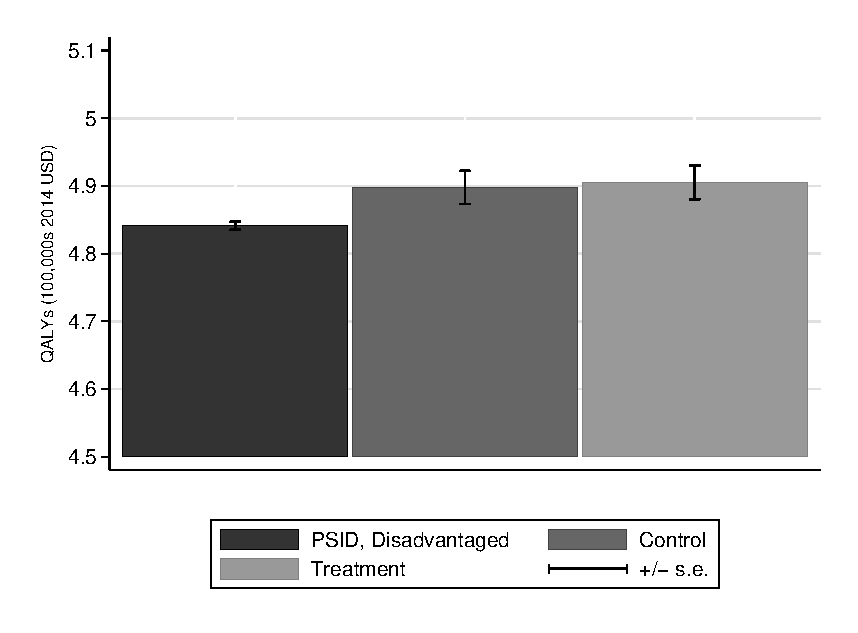
\includegraphics[width=\textwidth]{output/qalyexppsid_0.eps}
\end{subfigure}%
\begin{subfigure}[h]{0.5\textwidth}
	\centering
	\caption{Males} \label{fig:qpsid1}
		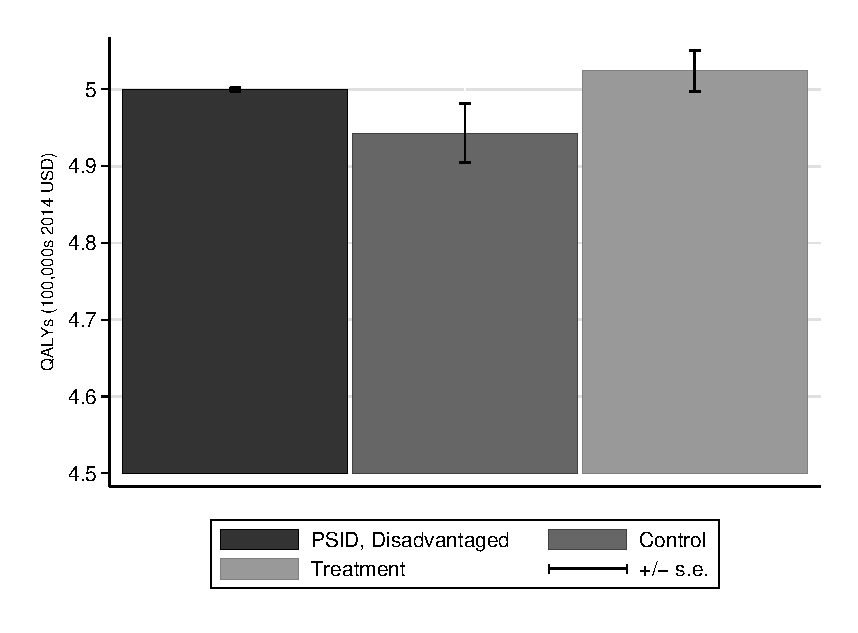
\includegraphics[width=\textwidth]{output/qalyexppsid_1.eps}
\end{subfigure}
\footnotesize \justify
Note: Panels (a) and (b) display the life-cycle net-present value of predicted quality-adjusted life years (QALYs) for ABC/CARE females and males, respectively, by treatment status. The predictions are based on combining data from the Panel Study of Income Dynamics (PSID), the Health Retirement Study, the Medical Expenditure Panel Survey (MEPS), and the Medicare Current Beneficiary Survey (MCBS). Each panel displays a comparison to to disadvantaged females and males in the Panel Study of Income Dynamics (PSID), where disadvantaged is defined as being black and having 12 years of education or less. QALYs are the quality-adjusted life years gain due to better health conditions. Standard errors are based on the empirical bootstrap distribution.\\
\end{sidewaysfigure}

\subsection{Crime}  \label{sec:crime}

To estimate the life-cycle benefits and costs of ABC/CARE related to criminal activity, we use rich data on crime outcomes.\footnote{Two previous studies consider the impacts of ABC on crime: \citet{Clarke_Campbell_1998_ABC_Comparison_ECRQ} use administrative crime records up to age 21, and find no significant differences between the treatment and the control groups. \cite{Barnett_Masse_2002_benefitcost,Barnett_Masse_2007_EER} account for self-reported crime at age 21. They find little effects, but the lack longer term, administrative data.} See Appendix \ref{appendix:crime} for a more complete explanation of the following procedures. We consider the following types of crime: arson, assault, burglary, fraud, larceny, miscellaneous (which includes traffic and non-violent drug crimes), murder, vehicle theft, rape, robbery, and vandalism. We use administrative data that detail: (i) youth arrests, gathered at the age-21 follow-up; (ii) adult arrests, gathered at the age-34 follow-up; and (iii) sentences, gathered at the age-34 follow-up. We also use self-reported data on adult crimes, gathered in the age-21 and age-30 subject interviews. Because none of these sources capture all criminal activity, it is necessary to combine them to more completely approximate the crimes the subjects committed. We also use several auxiliary datasets to complete the life-cycle profile of criminal activity and compute the costs of the committed crimes

We follow four steps to estimate the costs of crime.

\begin{enumerate}
\item \textit{Count arrests and sentences.} We start by counting the total number of sentences for each individual and type of crime (arson, assault, etc.) up to age 34, matching crimes across data sources, to construct the total number of  arrests for each individual and type of crime up to age 34.\footnote{In practice, we count all offenses (an arrest might include multiple offenses). This gives the correct number of victims for our estimations. The youth data have coarser categories than the rest of the data: violent, property, drug, and other. To match these data with the adult data, we assume that all property crimes were larcenies and that all violent crimes are assaults. In the ABC/CARE sample, assault is the most common type of violent crime, and larceny/theft is the most common property crime.} For individuals missing arrest data,\footnote{About 10\% of the ABC/CARE sample has missing arrest data. We fail to reject differences in observed characteristics between the treatment- and control-group participants for whom we observe arrests data (see Appendix~\ref{appendix:data}).} we impute the number of arrests by multiplying the number of sentences for each type of crime by a national arrest-sentence ratio for the respective crime.\footnote{This arrest-sentence ratio is constructed using the National Crime Victimization Survey (NJRP) and and the Uniform Crime Reporting Statistics (UCRS).}

\item \textit{Construct predictions.} Based on the sentences observed before age 34, we predict the sentences that the ABC/CARE subjects will have after age 34. Data from the North Carolina Department of Public Safety (NCDPS), which provide lifetime sentences of individuals in North Carolina, are used to estimate sentences incurred after age 34 from sentences incurred before age 34. Applying these models to the ABC/CARE data, we predict the number of future sentences for each subject up to age 50.\footnote{We assume that individuals with no criminal records before age 34 commit no crimes after age 34.} We then add these estimates to the original number of sentences, getting an estimate of the lifetime sentences. Adding these estimates increases the total count of crimes by 30\%--50\%.

\item \textit{Estimate number of victims from the crimes.} We only observe crimes that resulted in consequences in the justice system: crimes that resulted in arrests and/or sentences. To include unobserved crimes, we use victimization inflation (VI).\footnote{Previous papers using this method include \citet{Belfield_Nores_etal_2006_JHR} and \cite{Heckman_Moon_etal_2010_RateofReturn}.} We start by constructing a VI ratio, which is the national ratio of victims and arrests for each type of crime.\footnote{We assume that each crime with victims is counted separately in the national reports on arrests, even for arrests that might have been motivated by more than one crime. This victim-arrest ratio is constructed using the NJRP and the National Crime Victimization Survey (NCVS).} Then, we estimate the number of victims from the crimes committed by ABC/CARE subjects as their total arrests multiplied by the VI ratio.\footnote{Additionally, we can calculate an analogous estimate of the number of crime victims using sentences, based on the VI ratio and the national arrests-to-sentences ratio. Both estimates are very similar, as shown in Appendix \ref{appendix:crime}. To improve precision, the estimates in the rest of our paper are based on the average of the two calculations.}

\item \textit{Find total costs of crimes.} We use the estimates of the cost of crimes for victims from \cite{McCollister_etal_2010_DAD} to impute the total victimization costs. For crimes resulting in arrests and/or sentences, we consider justice system costs as well, such as police costs.\footnote{To be able to assign costs to each type of crime, we assume that the cost of the justice system depends on the number of offenses of each type, rather than on the number of arrests. While this could very slightly overestimate justice system costs, the costs only represent about 5\% of the total crime costs.} Finally, we construct the total costs of incarceration for each subject using the total prison time and the cost of a day in prison.
\end{enumerate}

\subsection{Education}

Follow-up data on educational attainment were collected up to age 30. In Appendix \ref{appendix:education}, we show that using auxiliary data sources, education up to this age is an accurate portrayal of lifetime educational attainment. Therefore, we do not predict beyond age 30. To monetize the costs of education, we consider the public costs of K-12 education and the private costs of post-secondary education, including vocational programs and community college. Other costs of education include grade retention and special education.

\section{Cost/benefit Analysis} \label{section:cbaresults}

This section reports cost/benefit and rate of return analyses underlying Figure~\ref{figure:npvsall}. The results we discuss are the central focus of this paper.

\subsection{Program Costs} \label{section:programscosts}

The yearly cost of the program was \$18,514 per participant in 2014 USD. We improve on previous cost estimates using primary-source documents.\footnote{Our calculations are based on progress reports written by the principal investigators and related documentation recovered in the archives of the research center where the program was implemented. We display these sources in Appendix \ref{app:programcosts}. The main component is related to staff costs. Other costs arise from nutrition and services that the subjects received when they were sick, diapers during the first 15 months of their lives, and transportation to the center. The control-group children also received diapers during approximately 15 months, and iron-fortified formula. The costs are based on sources describing ABC treatment for $52$ children. We use the same costs estimates for CARE, for which information is less available. The costs exclude any expenses related to research or policy analysis. Our calculation of the costs per year in 1979 USD is $\$295,239$. A separate calculation of the program as implemented indicates that the yearly cost of the program was $\$275,475$ (1979 USD). See Appendix \ref{app:programcosts}.}

\subsection{Non-experimental Data Sources}

To construct cost-benefit estimates we (i) \textit{interpolate} components not observed due to intermittent data collection; and (ii) \textit{extrapolate} (predict) components not observed because the follow-ups stop when the subjects were in their mid-30s. We use multiple sources of non-experimental data representative on the national or state level to construct these interpolations and extrapolations. Table~\ref{table:sources} presents the components for which we do these exercises and the sources we use.

\begin{table}[!htbp]
\begin{threeparttable}
\caption{Auxiliary Data Sources for Interpolation and Extrapolation of Life-cycle Benefits and Costs} \label{table:sources}
\footnotesize
%\input{../../AuxilliaryFiles/Preamble}
%\newgeometry{margin=.1in}

%\newcolumntype{L}[1]{>{\raggedright\let\newline\\\arraybackslash\hspace{0pt}}m{#1}}
%\newcolumntype{C}[1]{>{\centering\let\newline\\\arraybackslash\hspace{0pt}}m{#1}}
%\newcolumntype{R}[1]{>{\raggedleft\let\newline\\\arraybackslash\hspace{0pt}}m{#1}}

\begin{tabular}{L{3cm} C{1cm} C{1cm} C{1cm} C{1cm} C{1cm} C{2cm}} \toprule
 & \multicolumn{6}{c}{Subject's Age} \\
\textbf{Component}  & 16--21 & 21--30 & 31--34 & 34--50 & 61--67 & 68--Death \\ \midrule
\textbf{Transfer Income} & & \multicolumn{1}{c}{\cellcolor[gray]{.8} cNLSY} & \multicolumn{3}{c}{\cellcolor[gray]{.7} NLSY79; PSID}  &  \\ \midrule
\textbf{Subject Income} & &  \multicolumn{1}{c}{\cellcolor[gray]{.8} cNLSY} & \multicolumn{3}{c}{\cellcolor[gray]{.7} NLSY79; PSID} & \\ \midrule
\textbf{Health}  & \multicolumn{6}{c}{\cellcolor[gray]{.8} PSID; MEPS; MCBS; HRS}     \\ \midrule
\textbf{Crime} & \multicolumn{4}{c}{\cellcolor[gray]{.8} NCDPS; NJRP; NVS; UCRS} \\ \bottomrule
\end{tabular}
%\end{document}
\begin{tablenotes}
\footnotesize
Note: This table details the non-experimental data sources we use to interpolate and extrapolate the life-cycle benefits and costs of ABC/CARE. CNLSY: Children of the National Longitudinal Survey of the Youth 1979; NLSY79: National Longitudinal Survey of the Youth 1979; PSID: Panel Study of Income Dynamics; MEPS: Medical Expenditure Panel Survey; MCBS: Medicare Current Beneficiary Survey; HRS: Health and Retirement Study; NCDPS: North Carolina Department of Public Safety Data; NVS: National Crime Victimization Survey; NJRP: National Judicial Reporting Program; UCRS: Uniform Crime Reporting Statistics.
\end{tablenotes}
\end{threeparttable}
\end{table}

Figure~\ref{figure:npvs} presents the net present values for the main components of the cost/benefit analysis pooling males and females. The ``Baseline'' bars represent the estimates based on the first parameter of interest, comparing the treatment- to the control-group subjects. The ``Stay at Home'' bars represent the comparison between the treatment-group and the control-group subjects who stayed at home. The ``Alternative Preschool'' bars represent the comparison between the treatment-group and the control-group subjects who attended alternative preschools.

The first category, ``Costs," represents the cost of the programs' implementation. The second category, ``Total Net Benefits" quantifies the benefits for the treatment-group subjects net of the benefits of the control-group subjects. We consider labor income of both the participants and of their parents, ``Labor Income" and ``Parental Income." The program produces a positive net present value on labor income of the treated subjects. This considers income from age 21 all the way to retirement. 

We also account for the fact that the parents of the treatment-group subjects increased their labor supply and therefore their income. Ideally, we would like to consider the full life-cycle of parental income to allow for the possibility of wage growth induced by the education and work-experience accumulated while the childcare component of ABC/CARE. Especially because Table~\ref{table:tescombined} shows sizable and significant effects on parental income up to when the children are age 21. In practice, it is not feasible to find an auxiliary dataset allowing us to predict the income of parents with the observed characteristics of the children who attended ABC/CARE. The information we observe from the parents is too limited to produce a sensible prediction without using their children's characteristics. We take a more conservative approach and linearly interpolate parental labor income from chidren's cages 0 to 21, noting that we observe parental income at ages 1.5, 3.5, 4.5, 8, 12, 15, and 21.\footnote{Treatment effects for parental income at each of these ages are in Appendix~\ref{appendix:results}.}

Crime is an important component, which is consistent with previous analysis of early childhood education programs.\footnote{\citet{Heckman_Moon_etal_2010_RateofReturn}.} We then present two main categories for health, ``QALYs" and ``Medical Costs." As documented in \citet{Campbell_Conti_etal_2014_EarlyChildhoodInvestments}, ABC/CARE had substantial effects on several measures of long-term health, especially for males---e.g. body-mass index, systolic and diastolic pressure, Framigham risk index. This translates into a higher probability of survival at later ages. Thus, individuals in the treatment group incur higher medical costs. However, their health conditions enable them to have higher quality lives, which is reflected in the net gain the program generates in the QALYs. Finally, we present the net present value of education costs. It is negative because subjects in the treatment group acquired more education throughout their life cycles.

It is important to note that although the net present values from the three comparisons imply that ABC/CARE is socially beneficial regardless of control substitution, the magnitudes for some of the components do vary substantially. We argue that this has to do with the differential treatment effects of ABC/CARE by gender. As Figure~\ref{figure:npvsf} and Figure~\ref{figure:npvsm} show, males benefit much more when the counterfactual scenario is to attend alternative preschools, while females benefit much more from the program when the counterfactual scenario is to stay at home.

\begin{sidewaysfigure}[!htbp]
\caption{Life-cycle Net Present Value of Main Components of the CBA, Pooled Sample of Males and Females}
\label{figure:npvs}
\centering
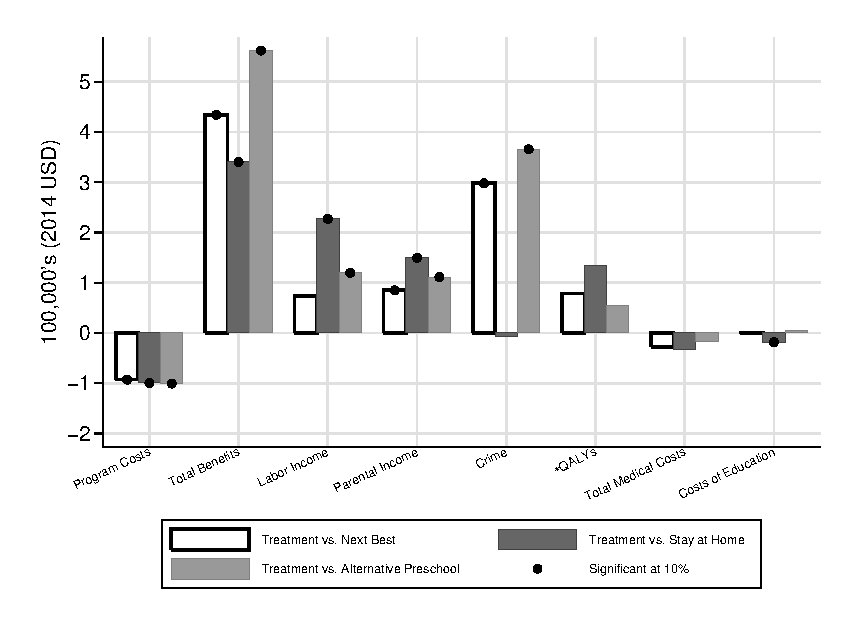
\includegraphics[width=.7\columnwidth]{output/abccare_npvs3.eps}
\floatfoot{
\footnotesize
Note: This figure displays the life-cycle net present values of the main components of the cost/benefit analysis of ABC/CARE from birth to age 79, discounted to birth at a rate of 3\%. ``Treatment vs. Control'': compares the treatment to the control group. ``Treatment vs. Stay at Home'': compares the treatment group to those subjects who stayed at home. ``Treatment vs. Alternative Preschool'': compares the treatment group to those subjects who attended alternative preschools. The latter two are based on matching estimators that account for selection on observable variables. By ``net" we mean that each component represents the total value for the treatment group minus the total value for the control group. Program costs: the total cost of implementing ABC/CARE. Total net benefits: the total net benefits of \textit{all} the components we consider. Labor income: total individual labor income from ages 20 to the retirement of program participants  (assumed to be age 67). Parental income: total parental labor income of the parents of the program participants from when the participants were ages 1.5 to 21. Crime: the total cost of crime (judicial and victimization costs). Total medical costs: both private and public medical costs from ages 15 to 79. Costs of education: the total costs of education of the individual from ages 6 to 26 and include any costs from special education and grade retention. The crime life-cycle net present value for Treatment vs. Stay at Home is different than zero. It is $-\$20,251.68$ (2014 USD). Inference is based on non-parametric, one-sided $p$-values from the empirical bootstrap distribution. We highlight point estimates significant at the $10\%$ level.\\
*QALYs refers to the quality-adjusted life years. Any gain corresponds to better health conditions through age 79.\\
}
\end{sidewaysfigure}

\begin{sidewaysfigure}[!htbp]
\caption{Life-cycle Net Present Value of Main Components of the CBA, Females}
\label{figure:npvsf}
\centering
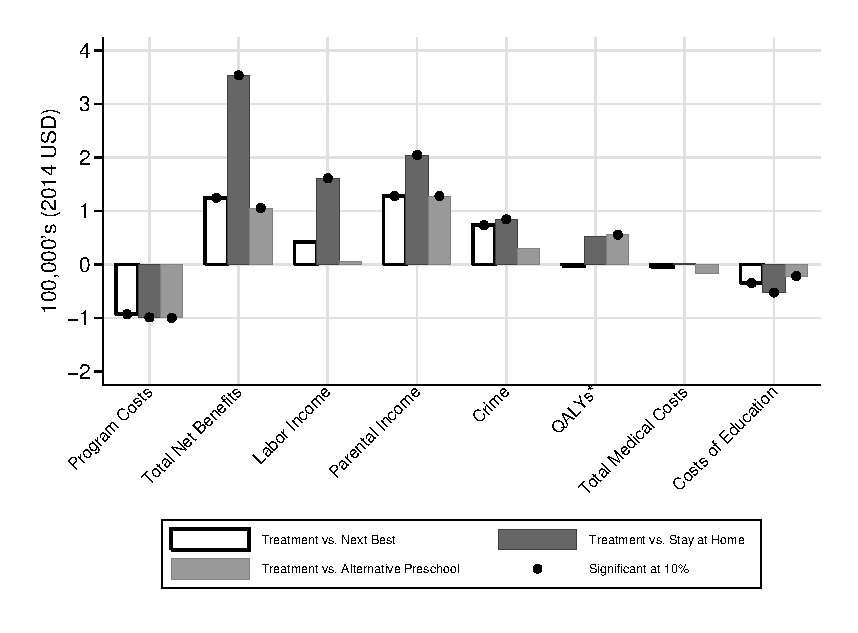
\includegraphics[width=.7\columnwidth]{output/abccare_npvs1.eps}
\floatfoot{
\footnotesize
Note: This figure displays the life-cycle net present values of the main components of the cost/benefit analysis of ABC/CARE from birth to age 79, discounted to birth at a rate of 3\%. ``Treatment vs. Control'': compares the treatment to the control group. ``Treatment vs. Stay at Home'': compares the treatment group to those subjects who stayed at home. ``Treatment vs. Alternative Preschool'': compares the treatment group to those subjects who attended alternative preschools. The latter two are based on matching estimators that account for selection on observable variables. By ``net" we mean that each component represents the total value for the treatment group minus the total value for the control group. Program costs: the total cost of implementing ABC/CARE. Total net benefits: the total net benefits of \textit{all} the components we consider. Labor income: total individual labor income from ages 20 to the retirement of program participants  (assumed to be age 67). Parental income: total parental labor income of the parents of the program participants from when the participants were ages 1.5 to 21. Crime: the total cost of crime (judicial and victimization costs). Total medical costs: both private and public medical costs from ages 15 to 79. Costs of education: the total costs of education of the individual from ages 6 to 26 and include any costs from special education and grade retention. Inference is based on non-parametric, one-sided $p$-values from the empirical bootstrap distribution. We highlight point estimates significant at the $10\%$ level.\\
*QALYs refers to the quality-adjusted life years. Any gain corresponds to better health conditions through age 79.\\
}
\end{sidewaysfigure}

\begin{sidewaysfigure}[!htbp]
\caption{Life-cycle Net Present Value of Main Components of the CBA, Males}
\label{figure:npvsm}
\centering
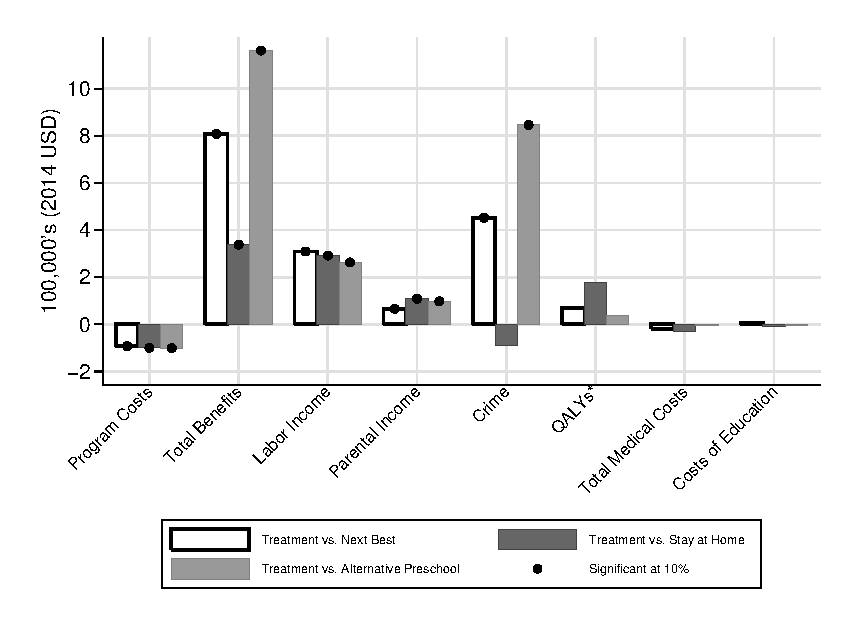
\includegraphics[width=.7\columnwidth]{output/abccare_npvs2.eps}
\floatfoot{
\footnotesize
Note: This figure displays the life-cycle net present values of the main components of the cost/benefit analysis of ABC/CARE from birth to age 79, discounted to birth at a rate of 3\%. ``Treatment vs. Control'': compares the treatment to the control group. ``Treatment vs. Stay at Home'': compares the treatment group to those subjects who stayed at home. ``Treatment vs. Alternative Preschool'': compares the treatment group to those subjects who attended alternative preschools. The latter two are based on matching estimators that account for selection on observable variables. By ``net" we mean that each component represents the total value for the treatment group minus the total value for the control group. Program costs: the total cost of implementing ABC/CARE. Total net benefits: the total net benefits of \textit{all} the components we consider. Labor income: total individual labor income from ages 20 to the retirement of program participants  (assumed to be age 67). Parental income: total parental labor income of the parents of the program participants from when the participants were ages 1.5 to 21. Crime: the total cost of crime (judicial and victimization costs). Total medical costs: both private and public medical costs from ages 15 to 79. Costs of education: the total costs of education of the individual from ages 6 to 26 and include any costs from special education and grade retention. Inference is based on non-parametric, one-sided $p$-values from the empirical bootstrap distribution. We highlight point estimates significant at the $10\%$ level.\\
*QALYs refers to the quality-adjusted life years. Any gain corresponds to better health conditions through age 79.\\
}
\end{sidewaysfigure}

We analyze the internal rate of return and benefit/cost ratio implied by the net present values presented in Figure~\ref{figure:npvs} through Figure~\ref{figure:npvsm}. The results without accounting for control substitution are presented in Table~\ref{table:cba}. All the monetary figures are in 2014 USD and are discounted to each child's birth, at a $3\%$ discount rate.\footnote{We present sensitivity analysis to different discount rates in Table~\ref{table:cba} and in Appendix~\ref{appendix:sensitivity}.} 

Pooling males and females, the results indicate that the program is socially efficient: the baseline estimates for the internal rate of return and the benefit/cost ratio are \irrp\ and \bcp. \textit{The program generates a benefit of \bcp\ for every dollar spent on it}. This is of particular importance because ABC/CARE was much more expensive than other early childhood education programs---the treatment involved more services over a longer time period \citep{Elango_Hojman_etal_2016_Early-Edu}.

The conclusion of statistically significant and beneficial internal rates of return and benefit/cost ratios are robust to deleting entire components of the benefit streams. First, we remove the component due to increased parental income. ABC/CARE had a childcare subsidy component allowing the mothers to work. This component amounts to \parincomenpvp. Even after removing this component, the internal rate of return and benefit/cost ratio indicate social efficiency of the program and remain statistically significant.

Parental income and crime are the components for which the internal rate of return and the benefit/cost ratio are the most sensitive. The reason for the sensitivity to parental income is that the amount is substantial and it is not heavily discounted because it substantially accumulates during the first $21$ years of the children's life. Crime occurs later in life and its benefits are accordingly discounted. The amount due to crime savings is large so removing it diminishes both the internal rate of return and the benefit/cost ratio (but they remain statistically significant).

The estimates are robust to individually removing the rest of the components, and in most cases remain statistically significant. This happens for one of either two reasons: (i) the effects are substantial but they are heavily discounted because they happen later in life---e.g. labor income; or (ii) the effects happen early in life but are not as substantial---as in the amount that the control-group parents pay for their children to attend alternative preschools.

Next, we analyze the estimates when splitting the sample by males and females. Some of the estimates loose significance due to the reduction of observations after splitting the sample by gender. The point estimates remain robust across  the sensitivity analysis (see Table~\ref{table:cba}), which computes the benefit/cost ratio and the internal rate of return when removing a component. For females, we observe consistency except for the case where we remove the parental income component. We can observe that the female sample is the main driver of parental income when comparing its net present value between females and males. For males, the estimates are robust, similar to the female sample.

\begin{table}[!htbp]
\centering
\caption{Cost/benefit Analysis of ABC/CARE, Summary}\label{table:cba}
\begin{adjustbox}{max width=\textwidth}
\begin{threeparttable}
\begin{tabular}{l r r r r r r r r r}																			
\toprule																			
&       \mc{3}{c}{Females}      &       \mc{3}{c}{Males}        &       \mc{3}{c}{Pooled}       \\																			
\cmidrule(lr){2-4}      \cmidrule(lr){5-7}      \cmidrule(lr){8-10}																			
Removed Component       &       NPV     &       IRR     &       B/C     &       NPV     &       IRR     &       B/C     &       NPV     &       IRR     &       B/C     \\																			
\midrule																			
None	&	161,759	&	\textbf{10.1\%}	&	\textbf{2.61}	&	919,049	&	\textbf{14.7\%}	&	\textbf{10.19}	&	636,674	&	\textbf{13.7\%}	&	\textbf{7.33}	\\
	&		&	(6\%)	&	(0.73)	&		&	(4\%)	&	(2.93)	&		&	(3\%)	&	(1.84)	\\ \\
Parental Income	&	148,854	&	4\%	&	1.12	&	107,907	&	\textbf{11\%}	&	\textbf{9.10}	&	116,953	&	\textbf{9\%}	&	\textbf{6.17}	\\
	&		&	(2\%)	&	(0.65)	&		&	(3\%)	&	(2.92)	&		&	(3\%)	&	(1.87)	\\
Subject Labor Income	&	41,908	&	9\%	&	\textbf{2.21}	&	238,105	&	\textbf{13\%}	&	\textbf{7.75}	&	133,032	&	\textbf{13\%}	&	\textbf{6.03}	\\
	&		&	(6\%)	&	(0.66)	&		&	(5\%)	&	(2.23)	&		&	(4\%)	&	(1.77)	\\
Subject Transfer Income	&	419	&	\textbf{10\%}	&	\textbf{2.61}	&	-7,265	&	\textbf{15\%}	&	\textbf{10.26}	&	-4,372	&	\textbf{14\%}	&	\textbf{7.38}	\\
	&		&	(6\%)	&	(0.73)	&		&	(4\%)	&	(2.93)	&		&	(3\%)	&	(1.84)	\\
Subject QALY	&	42,102	&	9\%	&	\textbf{2.20}	&	106,218	&	\textbf{14\%}	&	\textbf{9.14}	&	87,181	&	\textbf{13\%}	&	\textbf{6.48}	\\
	&		&	(6\%)	&	(0.69)	&		&	(6\%)	&	(2.73)	&		&	(5\%)	&	(1.79)	\\
Medical Expenditures	&	-16,037	&	9\%	&	\textbf{2.77}	&	-42,038	&	\textbf{15\%}	&	\textbf{10.61}	&	-31,221	&	\textbf{14\%}	&	\textbf{7.65}	\\
	&		&	(6\%)	&	(0.76)	&		&	(3\%)	&	(2.89)	&		&	(3\%)	&	(1.85)	\\
Alternative Preschools	&	16,691	&	8\%	&	\textbf{2.45}	&	13,434	&	\textbf{14\%}	&	\textbf{10.05}	&	14,659	&	\textbf{12\%}	&	\textbf{7.19}	\\
	&		&	(5\%)	&	(0.73)	&		&	(4\%)	&	(2.92)	&		&	(3\%)	&	(1.84)	\\
Education Costs	&	1,457	&	\textbf{10\%}	&	\textbf{2.59}	&	-7,852	&	\textbf{15\%}	&	\textbf{10.26}	&	-4,518	&	\textbf{14\%}	&	\textbf{7.37}	\\
	&		&	(6\%)	&	(0.72)	&		&	(4\%)	&	(2.93)	&		&	(3\%)	&	(1.86)	\\
Crime Costs	&	31,668	&	10\%	&	\textbf{2.34}	&	638,923	&	\textbf{9\%}	&	4.08	&	450,368	&	\textbf{8\%}	&	\textbf{3.06}	\\
	&		&	(6\%)	&	(0.62)	&		&	(5\%)	&	(2.18)	&	&	(4\%)	&	(1.01)	\\ \\
Deadweight Loss	&		&	\textbf{18\%}	&	\textbf{3.83}	&		&	\textbf{19\%}	&	\textbf{15.38}	&		&	\textbf{18\%}	&	\textbf{11.01}	\\
	&		&	(12\%)	&	(1.04)	&		&	(6\%)	&	(4.35)	&		&	(5\%)	&	(2.79)	\\
0\% Discount Rate	&		&		&	\textbf{5.06}	&		&		&	\textbf{25.45}	&		&		&	\textbf{17.40}	\\
	&		&		&	(2.82)	&		&		&	(10.42)	&		&		&	(5.90)	\\
7\% Discount Rate	&		&		&	\textbf{1.49}	&		&		&	\textbf{3.78}	&		&		&	\textbf{2.91}	\\
	&		&		&	(0.32)	&		&		&	(0.79)	&		&		&	(0.59)	\\
\bottomrule																			
\end{tabular}																			

\begin{tablenotes}
\footnotesize
\item Note: This table presents the estimates of the net present value (NPV) for each component, and the internal rate of return (IRR) and the benefit/cost ratio (B/C) of ABC/CARE for different scenarios based on comparing the groups randomly assigned to receive center-based childcare and the groups randomly assigned as control in ABC/CARE. The first row represents the baseline estimates. The rest of the rows present estimates for scenarios in which we remove the NPV estimates of the component listed in the first column. Alternative Preschools refer to money spent in alternatives to treatment from the control-group children parents. QALYs refers to the quality-adjusted life years. Any gain corresponds to better health conditions through age 79. The quantity listed in the NPV columns is the component we actually remove when computing the calculation in each row. All the money figures are in 2014 USD and are discounted to each child's birth, unless otherwise specified. For the B/C we use a discount rate of $3\%$, unless otherwise specified. We test the null hypotheses $\text{IRR} = 3\%$ and $\text{B/C} = 1$---we elect $3\%$ because that is the discount rate we use. Inference is based on non-parametric, one-sided $p$-values from the empirical bootstrap distribution. We highlight point estimates significant at the $10\%$ level.
\end{tablenotes}
\end{threeparttable}
\end{adjustbox}
\end{table}

We provide a cost/benefit analysis of the program when accounting for control substitution (Table~\ref{table:cbacs}). The first row shows the estimates without accounting for control substitution, i.e. the same as those of the first row in Table~\ref{table:cba}. The second and third rows present results for the two counterfactual comparisons we consider throughout the paper. The results are consistent with the treatment effects we show in Section~\ref{section:c-functions}. Compared to ABC/CARE, females benefit more than males from alternative preschools relative to staying at home. That is, the benefit/cost ratio of ABC/CARE relative to staying at home is high for females and low for males. Conversely, the benefit/cost ratio of ABC/CARE relative to alternative preschools is high for males and low for females. The gender-difference in results is consistent with two facts elsewhere noted: (i) stark outcome gender differences caused from attending childcare \citep{Kottelenberg-Lehrer_2014_Gender-Effects,Baker_Gruber_Milligan_2015_Noncog_Defects,Doyle-etal_2015_Econ-Hum-Bio,Doyle-etal_2016_PLoS-ONE}; and (ii) girls being less sensitive to uncertain environments \citep{Autor-etal_2015_Family-Disadvantage}.

\begin{table}[!htbp]
\begin{threeparttable}
\caption{Cost/benefit Analysis Accounting for Control Substitution}
\label{table:cbacs}
\centering
\begin{tabular}{l c c c c c c }
\toprule
	&	\mc{2}{c}{Females}					&	\mc{2}{c}{Males}					&	\mc{2}{c}{Pooled}					\\
		\cmidrule(lr){2-3}						\cmidrule(lr){4-5}						\cmidrule(lr){6-7}					
Estimate 	&	IRR	&	B/C	&	IRR	&	B/C	&	IRR	&	B/C	\\
\midrule

% INSERT summary_tex.xls FILE BELOW
% INSERT summary_tex.xls FILE BELOW
% INSERT summary_tex.xls FILE BELOW

Baseline	&	0.10 	&	\textbf{2.59}	&	\textbf{0.14} &	\textbf{9.75} 	&	\textbf{0.13}	&	\textbf{5.58}	\\
	&	(0.07)	&	(0.97)	&	(0.05)	&	(4.59)	&	(0.05)	&	(2.32)	\\
Relative to Staying at Home	&	\textbf{0.15}	&	\textbf{4.81}	&	\textbf{0.09}	&	4.32	&	\textbf{0.10} &	\textbf{4.42}	\\
	&	(0.07)	&	(1.42)	&	(0.04)	&	(2.70)	&	(0.03)	&	(1.39)	\\
Relative to Alternative Preschools	&	0.10		&	\textbf{2.37}	&	\textbf{0.17}	&	\textbf{12.38}	&	\textbf{0.14}	&	\textbf{6.29}	\\
	&	(0.07)	&	(0.91)	&	(0.05)	&	(5.16)	&	(0.04)	&	(2.23)	\\

% INSERT summary_tex.xls FILE ABOVE
% INSERT summary_tex.xls FILE ABOVE
% INSERT summary_tex.xls FILE ABOVE

\bottomrule
\end{tabular}
\begin{tablenotes}
\footnotesize
\item Note: This table displays estimates of the internal rate of return (IRR) and the benefit/cost ratio (B/C) for ABC/CARE for three cases. Not accounting for control substitution (baseline); comparing ABC/CARE to staying at home (relative to staying at home); and comparing ABC/CARE to alternative preschools (relative to alternative preschools). For the B/C we use a discount rate of $3\%$. We test the null hypotheses $\text{IRR} = 3\%$ and $\text{B/C} = 1$---we elect $3\%$ because that is the discount rate we use. Inference is based on non-parametric, one-sided $p$-values from the empirical bootstrap distribution. We highlight point estimates significant at the $10\%$ level.
\end{tablenotes}
\end{threeparttable}
\end{table}

\subsection{Using our Estimates to Understand Recent Cost/benefit Analyses}

\noindent An example of the approach recent studies take on cost-benefit analyses is \citet{Kline_Walters_2016_QJE}. They use data of the Head Start Impact Study (HSIS) to evaluate Head Start and find that a benefit/cost ratio between $1.50$ and $1.84$.\footnote{HSIS is a one-year-long randomized evaluation of Head Start.} Their analysis contains three steps: (i) calculate the treatment effect on Wechsler Preschool and Primary Scale of Intelligence (WPPSI) at age 5; (ii) monetize this gain using the return to WPPSI at age 5 in terms of net present value of labor income at age 27 \citep{Chetty_Friedman_etal_2011_QJoE}.\footnote{For this comparison exercise, we interpret the earnings estimated in \citet{Chetty_Friedman_etal_2011_QJoE} to be equivalent to labor income.} Calculations from \citet{Chetty_Friedman_etal_2011_QJoE} indicate that a 1 standard deviation gain in WPPSI at age 5 implies a $13.1\%$ increase in the net present value of labor income at age 27;\footnote{This is based on combining information from Project Star and administrative data at age 27.} and (iii) calculate the benefit/cost ratio based on this gain and their own calculations of the program's cost. This calculation is based on assigning the net present value of labor income at age 27 of $\$385,907.17$ to the control-group participants, which is provided by  \citet{Chetty_Friedman_etal_2011_QJoE}.\footnote{All money values that we provide in this section are in 2014 USD. We discount the value provided by \citet{Chetty_Friedman_etal_2011_QJoE} to the age of birth of the children in our sample (first cohort).}


\begin{table}[!htbp]
\begin{threeparttable}
\caption{Alternative Cost-benefit Analyses Calculations}
\label{table:comparing}
\centering
\footnotesize

\begin{tabular}{cllcc}
\toprule
Age & \mc{1}{c}{NPV Source} & Component & \citet{Kline_Walters_2016_QJE} & Authors' Method \\
& & & Method & \\
\midrule
\multirow{2}{*}{27} & \cite{Chetty_Friedman_etal_2011_QJoE} & Labor income & 0.58 (s.e. 0.28) &  \\
& ABC/CARE-calculated & Labor income & 0.09 (s.e. 0.04) &  1.09 (s.e. 0.04)\\
\midrule
\multirow{2}{*}{34} & ABC/CARE-calculated & Labor income & 0.37 (s.e. 0.04) & 0.15 (s.e. 0.05) \\
& ABC/CARE-calculated & All & 1.21 (s.e. 0.05) &  3.20 (s.e. 1.04) \\
\midrule
\multirow{2}{*}{Life-cycle} &  ABC/CARE-calculated & Labor income & 1.56 (s.e. 0.08) & 1.55 (s.e. 0.76) \\
& ABC/CARE-calculated & All & 3.80 (s.e. 0.29) & 7.33 (s.e. 1.84) \\
\bottomrule
\end{tabular}

\begin{tablenotes}
\footnotesize
\item Note: This table displays benefit/cost ratios based on the methodology in \citet{Kline_Walters_2016_QJE} and based on our own methodology. Age: age at which we stop calculating the net-present value. NPV Source: source where we obtain the net present value. Component: item used to compute net present value (all refers to the net present value of all the components). \citet{Kline_Walters_2016_QJE} Method: estimate based on these authors methodology. Author's Method: estimates based on our methodology. Standard errors are based on the empirical bootstrap distribution.
\end{tablenotes}
\end{threeparttable}
\end{table}

To analyze how our estimates compares to the method in \citet{Kline_Walters_2016_QJE}, we present a series of exercises in the third column of Table~\ref{table:comparing}. For comparison, the fourth column of Table~\ref{table:comparing} displays the analogous exercise using our own method.

In the first exercise, we use both the ``return to WPPSI'' and the net-present value of labor income at age 27 in  \citet{Chetty_Friedman_etal_2011_QJoE}. In the second exercise, we perform a similar exercise but we use our own estimate of the net-present value of labor income at age 27.\footnote{This allows us to compute our own ``return to WPPSI'' and impute it to the treatment-group individuals.} The reminder of exercises are similar, but (i) vary the age up to where we consider the net-present value of labor income; (ii) consider the value of all the components we analyze throughout the paper; or (iii) both.

There are four gains from our methodology: (i) provides a more precise estimate of the net-present value (and the return to WPPSI) of the components, as our interpolation and extrapolation are based on matching our experimental sample to various non-experimental samples. We do not impute a net present value or a return of an \textit{ad hoc} experiment; (ii) better quantifies the effects of the analyzed experiment by considering the whole life-cycle; and (iii) better approximates the statistical uncertainty of our estimates by considering both the sampling error in the experimental and non-experimental samples and the prediction error due to the interpolation and extrapolation; (iv) enables for an extensive sensitivity analysis of each of the components we monetize.

\section{Summary} \label{section:conclusion}

We study two closely related early childhood education programs with randomized controlled design and provide a template to evaluate social programs solving a number of methodological and practical issues. These include non-compliance, attrition, multiple hypotheses testing, and the prediction of long-term outcomes. We provide a comprehensive evaluation by considering and summarizing the treatment effects for a multiplicity of outcomes. This have direct relationship with policy-relevant questions.

As a program providing high-quality center-based childcare, ABC/CARE has positive effects on a variety of outcomes measuring human development throughout childhood to adulthood---including cognition, socio-emotional skills, criminal activity, and adulthood health. This translates into statistically and economically significant measures of social efficiency, like the benefit-cost ratio and the internal rate of return, which we calculate accounting for complications that arise when evaluating social programs and considering life-cycle gains.

When adequately assessed, early childhood education programs enhance human development in that they provide a vehicle to promote social mobility. An adequate evaluation requires: (i) comparing the program with respect to a well-defined counterfactual---e.g. other programs or staying at home; and (ii) monetizing the life-cycle gains, which goes beyond back-of-the-envelope calculations based on short-term gains.

%References
\singlespace
\bibliographystyle{chicago}
\bibliography{heckman}

\end{document} 